%!TEX root = Bericht.tex
\graphicspath{{graphics/}}

\chapter{Trajectory Planning}
\label{cha:trajectory}
For the two most advanced modes, i. e. the Half-Automatic and the Full-Automatic Mode, trajectories had to be generated. In this chapter the best trajectories for \textsc{Skye} are elaborated and tested with suitable trajectory controllers. Performance results based on a \textsc{Matlab} simulation are shown.

%\subsection{Our Approach}
%From the GUI it was given that the goal trajectory would be a multipoint-interpolating %trajectory. The user is able to define waypoints on a map which afterwards should be %connected with a reasonable and realizable trajectory. Beside interpolating trajectories %there exist also approximating trajectories but they were not taken into consideration, since %usually the user wants skye fly directly through a waypoint.

\section{Experimental Design}
\label{sec:experimental design}
The main application fields of the system \textsc{Skye} are image capturing and agile performance demonstrations. The waypoints used to test the trajectory algorithms had therefore to be alike these situations. All the results below belong to the three sample waypoints shown in figure \ref{fig:sampleNodes}. They represent standard situations for the applications mentioned before. Indeed, to verify the conclusions, some a wider set of waypoints had to be considered.
\\
The first waypoints are similar as they would be set to capture images of the the university building. 

\begin{figure}[h]
  \begin{minipage}[t]{0.32\textwidth}
    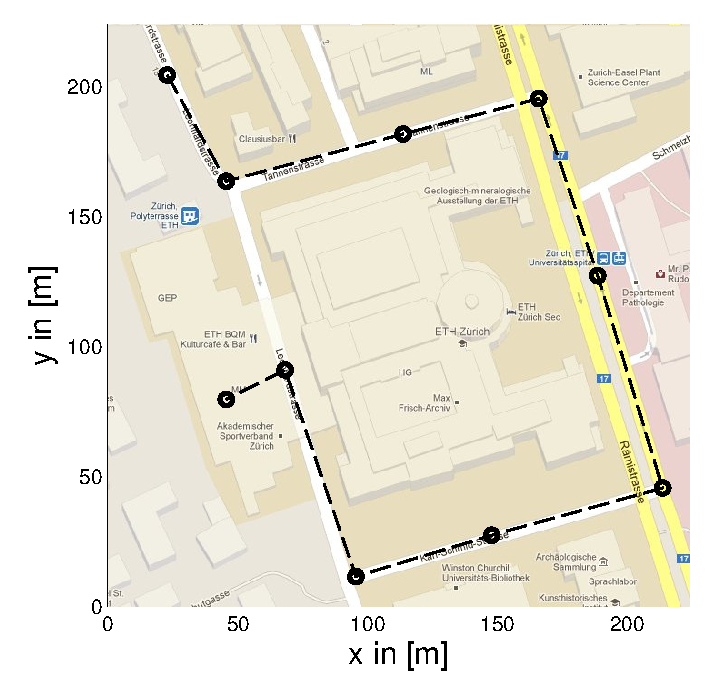
\includegraphics[width = \textwidth]{graphics/sampleNodeRoad}
  \end{minipage}
  \hfill
  \begin{minipage}[t]{0.32\textwidth}
    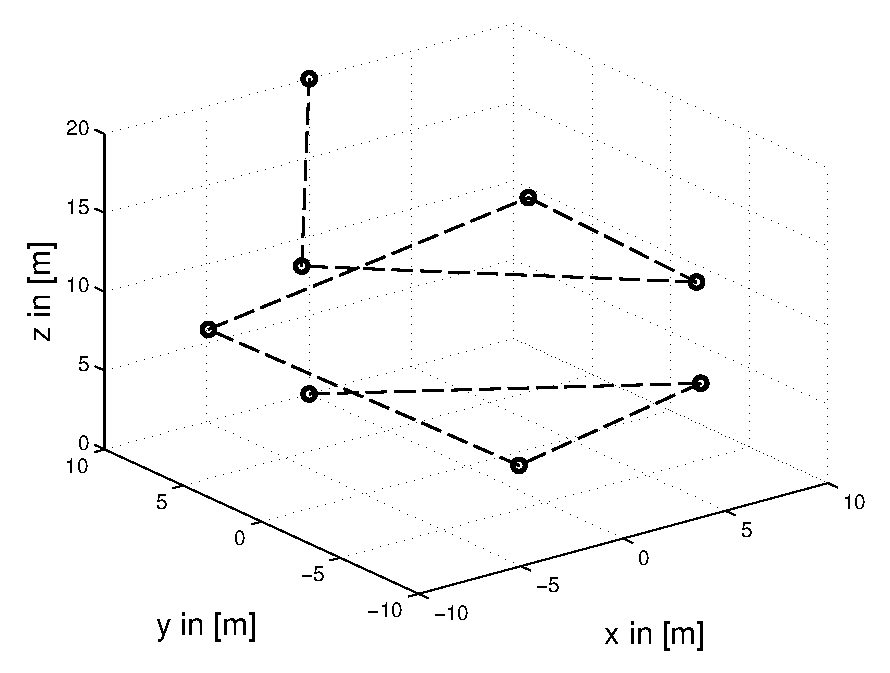
\includegraphics[width = \textwidth]{graphics/sampleNodeHelix}
  \end{minipage}
  \hfill
  \begin{minipage}[t]{0.32\textwidth}
    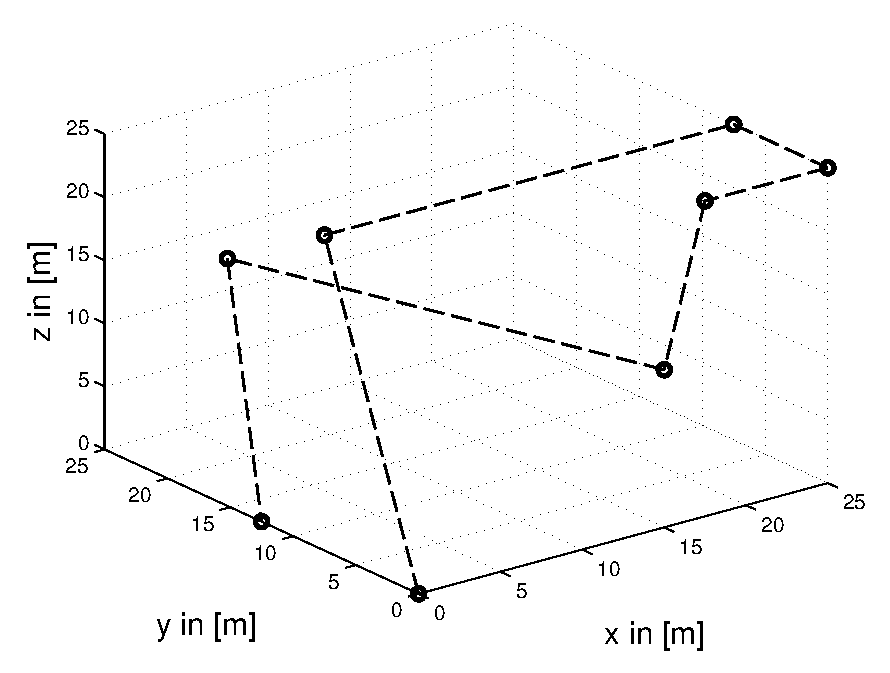
\includegraphics[width = \textwidth]{graphics/sampleNodeAgile}
  \end{minipage}
  \caption{The experimental environment based on three samples. {\bf Left:} The \textit{road} waypoints represent the need of low overshoots to not touch obstacles beside the streets. Its long straight ways enable high velocities. {\bf Center:} The \textit{helix} waypoints represents the circumnavigation of any obstacle. It yields to high curvatures of the track. {\bf Right:} The \textit{agile} waypoints include both straight sections as high curvatures.}
  \label{fig:sampleNodes}
\end{figure}


Furthermore, to score (\textbf{and optimize?}) the generated trajectories $\tilde{p}(t)$ and the resulting trace of the system $r(t)$, we set up the following criteria. Criteria (\ref{item:static_deviation}) to (\ref{item:static_acceleration}) are refered to as \textit{static criteria} as they do not depend any simulation. The remaining ones (\textit{dynamic criteria}) then mainly depend on the used controller\footnote{For detailed description of the used notation consider section \ref{sec:definition}}.
\\
Being $L_p$ the length of the path ${\bf p}(u)$ and $T_p$ the time of the trajectory $\tilde{\bf p}(t)$
\begin{equation}
L_p = \int_{u_{min}}^{u_{max}} du \qquad T_p = \int_{t_{min}}^{t_{max}} dt
\label{eq:length_of_path}
\end{equation}
the criteria are:

\begin{enumerate}[i)] 
\item Average deviation between actual path and chord connection between waypoints
\label{item:static_deviation}
\begin{equation}
J_1 = \int_{u_{min}}^{u_{max}} \|{\bf p}(u)- {\bf p}_2(u)\| du \cdot L_p^{-1} \label{eq:static_deviation}
\end{equation}

\item Average curvature of path\footnote{For a derivation of curvature see any vetor analysis book, e.g. \cite{stammbach} chapter II, page 71.}
\label{item:static_curvature}
\begin{equation}
J_2 = \int_{u_{min}}^{u_{max}} \frac{\| \frac{d {\bf p}}{du} \times \frac{d^{2} {\bf p}}{du^{2}} \|}{\|  \frac{d {\bf p}}{du} \|^3}du \cdot L_p^{-1}
\label{eq:static_curvature}
\end{equation}
% THIS ALTERNATIVE NOTATION IS INCONSEQUENCE IN USING DOT WHEN NOT HAVING PARAM T !!
% J_2 = \int_{u_{min}}^{u_{max}} \frac{\| \dot{\bf p}(u) \times \ddot{\bf p}(u) \|}{\| \dot{\bf p}(u) \|^3}du \cdot L_p^{-1}

\item Average acceleration of the trajectory
\label{item:static_acceleration}
\begin{equation}
J_3 = \int_{t_{min}}^{t_{max}} \|{\bf \ddot{\tilde{p}}}(t)\| dt \cdot T_p^{-1} \label{eq:static_acceleration}
\end{equation}

\item Deviation between trajectory and trace of the system\footnote{The deviation vector between trace and its closest point on the trajectory is always normal to the latter. Compare with figure \ref{fig:scene_crossTrack}.}
\label{item:dynamic_deviation}
\begin{equation}
J_4 = \int_{t_{min}}^{t_{max}} \| {\bf \tilde{p}}(t_{cl}) - {\bf r}(t) \| dt \cdot T_p^{-1} 
\label{eq:dynamic_deviation}
\end{equation}

\item Average acceleration of the system
\label{item:dynamic_acceleration}
\begin{equation}
J_5 = \int_{t_{min}}^{t_{max}} \|{\bf \ddot{r}}(t)\| dt \cdot T_p^{-1}
\end{equation}

\item Time synchronity\footnote{Time synchronity should be warranted for accurate \textit{trajectory} following. In our task for caputuring time independent imagery, it was only considered as a secondary aspect.}
\label{item:dynamic_synchronity}
\begin{equation}
J_6 = \| {\bf \tilde{p}}(t_{max}) - {\bf r}(t_{max}) \| \cdot L_p^{-1} \label{eq:dynamic_synchronity}
\end{equation}

\end{enumerate}


\section{Definition of Trajectories}
\label{sec:definition}
\subsection{Paths and Trajectories}
The main difference between a path $ {\bf p}(u)$ and a trajectory $ {\bf \tilde{p}}(t)$ is that only the latter includes time, i.e. considers the dynamics. A path is only defined as the way to go from point a to point b. Therefore it only has geometrical properties. In order to generate a trajectory, a time needs to be assigned to each point on the path. This is done with a function $u=u(t)$ that connects the parameter $u$ of the geometrical path with the time. The composition of the function\footnote{In  \cite{snider} named as the \textit{Motion Law}} $u=u(t)$ and the geometrical path ${\bf p}(u)$ finally forms the trajectory ${\bf \tilde{p}}(t)$. This concept is shown in figure \ref{fig:path_trajectory}.
\begin{figure}[h]
\centering
\def\svgwidth{0.9\textwidth}
\input{graphics/PathTrajectory.pdf_tex}
\caption{Composition of a path ${\bf p}(u)$ and the motion law $u(t)$ forming the trajectory ${\bf \tilde{p}}(t)$}
\label{fig:path_trajectory}
\end{figure}

In order to get the velocity and acceleration of the trajectory, the chain rule has to be applied to ${\bf \tilde{p}}(t)=({\bf p}\circ u)(t)$:

\begin{align}\label{vel_acc}
{\bf \dot{\tilde{p}}}(t) &= \frac{d {\bf p}}{du}\dot{u}(t) \\
{\bf \ddot{\tilde{p}}}(t) &= \frac{d {\bf p}}{du}\ddot{u}(t)+\frac{d^{2} {\bf p}}{du^{2}}\dot{u}^{2}(t)
\end{align}

%{\bf \ddot{\tilde{p}}}(t)





\subsection{Interpolation and Approximation}
If one wants to draw a path through a set of waypoints, there exists two ways to do this. First, the path can pass through all waypoints no matter how many bends it will have. Secondly, the path tries to best fit waypoint set, i.e. a function of a  certain order is adopted to best fit the waypoints. This can be done with different methods, e.g with least-squares. The first approach is called interpolation whereas the second approach is called approximation. Depending on the choice, different curves with different properties are formed (see figure \ref{fig:ApproxInterpol}).  


\begin{figure}[H]
  \begin{minipage}[t]{0.9\textwidth}
    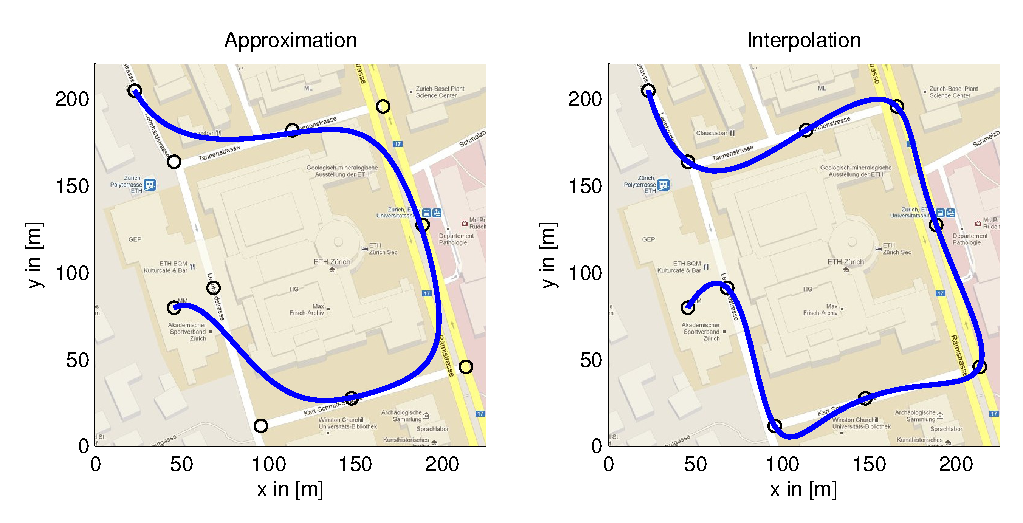
\includegraphics[width = \textwidth]{graphics/ApproxInterpol.eps}
  \end{minipage}
  \caption{Interpolation and approximation of waypoints}
  \label{fig:ApproxInterpol}
\end{figure}

For the the trajectory planning for \textsc{Skye}, it was necessary to interpolate the waypoints. This was due to the GUI used (see \ref{sec:realization}). There only a small amount of waypoints is set ant the pilot expects the UAV to pass through all of them and not to take a shortcut. The approximation of the waypoints could result in a collision with buildings as shown in \ref{fig:ApproxInterpol}.


There mainly exist two solution to interpolate a given set of $n+1$ waypoints. A polynomial (of order $\ge n+1$) from $\varPi_{n}$ or else a set of polynomials of lower order, defined over a certain interval, can be used. This set of polynomials finally forms a spline. As impressively shown in \cite{wolfgang}, splines are the better option for more than a few waypoints. 



\section{Splines}
\label{sec:splines}
\subsection{Parameterization}
Before actually a path can be drawn through a set of waypoints respectively a spline can be calculated, a value of the parameter $u$ needs to be assigned to all $n+1$ waypoints, i.e. a nondecreasing sequence of $u_0 < u_1 < ...< u_n$ must be found. In this section, the most common used techniques are analyzed\footnote{A vaster evaluation of different parameterizations can be found in \cite{haron}} The choice of parameterization affects the geometrical properties of the path on the one hand and the velocity and acceleration of the trajectory on the other hand. (compare \eqref{vel_acc}). Latter is especially of big impact if a proportional relation is used to describe the motion law, i.e. $u=\lambda t$ (compare \ref{sec:motionLaw}).

\subsubsection{Uniform}
This is the simplest way to define the $u_{0-n}$. Here basically the index number of the waypoints are assigned to $u$. Therefore no meaningful interpretation can be made.
\begin{equation*}
u_n-u_{n-1}=1
\end{equation*}
\subsubsection{Chord length}
In this method the chord length between the waypoints is calculated and then summed up and assigned to $u$. With $u=\lambda t$ this method can be interpreted to aim for a more or less constant velocity over the whole trajectory.
\begin{equation*}
u_n-u_{n-1}=\left \| \begin{bmatrix}x_n\\y_n\\z_n \end{bmatrix}-\begin{bmatrix}x_{n-1}\\y_{n-1}\\z_{n-1} \end{bmatrix}\right \|
\end{equation*}
\subsubsection{Arc length}
The arc length method is improved version of the chord length distribution in order to reach a constant velocity. Here instead of taking the chord length between two waypoints, the arc length is estimated and summed up. The algorithm\footnote{The algorithm was taken from \cite{engeln} and implemented in \textsc{Matlab}.} for that can be found in \ref{subsec:arcLengthDistribution}.

\begin{figure}[h]
\centering
\def\svgwidth{0.7\textwidth}
\input{graphics/arcLength.pdf_tex}
\caption{The arc length is estimated using the segments of two circles.}
\label{fig:arcLength}
\end{figure}

\begin{equation*}
u_n-u_{n-1}=\frac{B_a+B_b}{2}
\end{equation*}

\subsubsection{Centripetal}
This method was first proposed in \cite{lee}. Here the root of the chord length is used. The motivation for this method is that the larger the angular change from $\textnormal{waypoint}_{n-1}$ to $\textnormal{waypoint}_n$, the more centripetal force is accepted. A justification for this statement can be found in \cite{doessegger} and \cite{lee}.
\begin{equation*}
u_n-u_{n-1}=\sqrt{\left \| \begin{bmatrix}x_n\\y_n\\z_n \end{bmatrix}-\begin{bmatrix}x_{n-1}\\y_{n-1}\\z_{n-1} \end{bmatrix}\right \|}
\end{equation*}

\subsubsection{Discussion}

geometrical properties, dynamical properties, Kreb'sche Bewertungsalgrithmen:) \textbf{pictures of all of them, justify choice, say that if more waypoints, different decision}

All those four methods were tested on our three sample waypoints defined in \ref{sec:experimental design}. Since the helix waypoints all have the same distance between each other, all four methods result in the same path respectively trajectory. As the chord and arc length distribution try to maintain a constant velocity, it is obvious that high curvature has to be omitted. This however leads to overshoots as seen in \ref{fig:parameterizations4_road_agile}. Choosing cubic splines reduces this effect whereas quintic splines amplifies it. (compare \ref{fig:parameterization_cqq})

\begin{figure}[H]
  \begin{minipage}[t]{0.9\textwidth}
    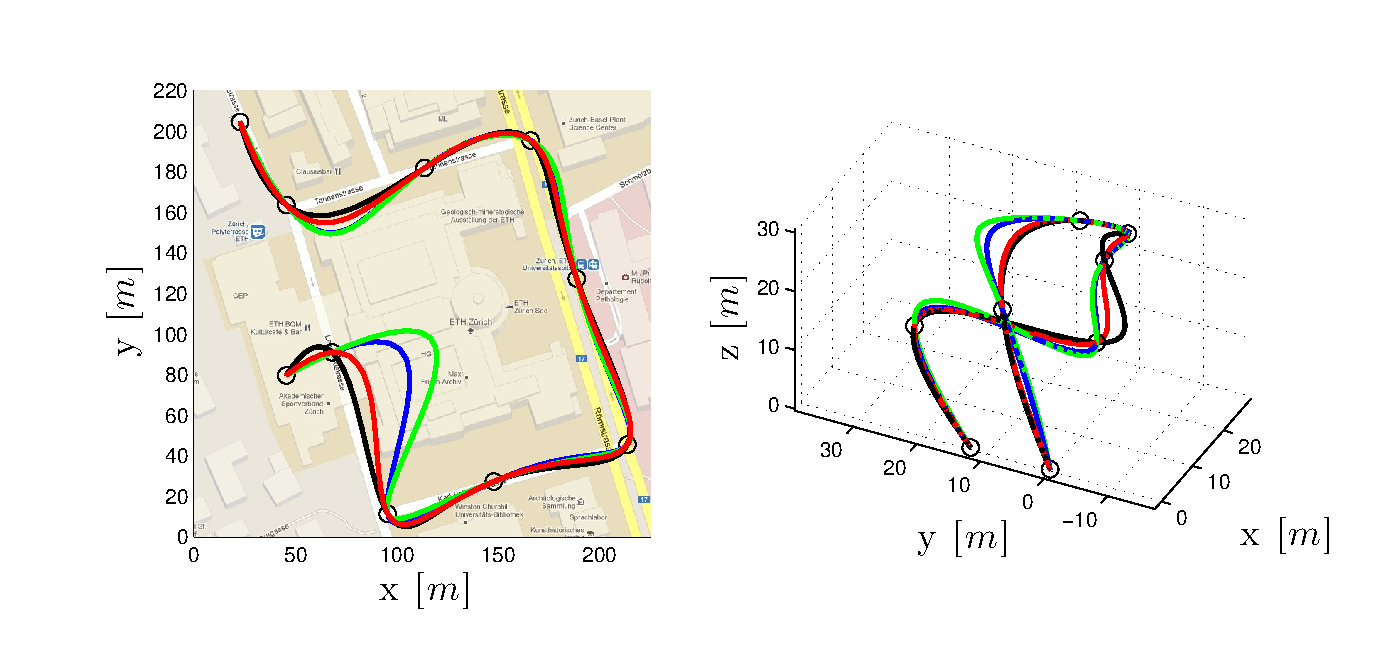
\includegraphics[width = \textwidth]{graphics/Parameterizations4_road_agile.eps}
  \end{minipage}
  \caption{The different parameterizations shown with quartic splines; Uniform:black, Chord length: blue, Arc length: green, Centripetal: red}
  \label{fig:parameterizations4_road_agile}
\end{figure}

Since those overshoots are intolerable a uniform or centripetal distribution has to be chosen. While in our sample waypoints the two seem to be quite similar the uniform distribution sometimes leads to  loops or cusps as shown in \cite{lee} and \cite{haron}. This occurs if the chord distance between the waypoints suddenly changes a lot, since the uniform distribution is completely independent of the waypoint set. Therefore the centripetal distribution was chosen to fit best our needs.
\\
Beside the geometrical appearance due to the different distributions the dynamic properties are also of big interest if a constant time scaling is used, as described in \ref{subsec:timeScaling}. Here, as the centripetal distribution is already chosen due to its geometrical properties, this is only shown for reasons of completeness. However, if the waypoints were set in a closer succession the geometrical properties would not be that important anymore and the decision should be rethought.

\begin{figure}[H]
  \begin{minipage}[t]{0.96\textwidth}
    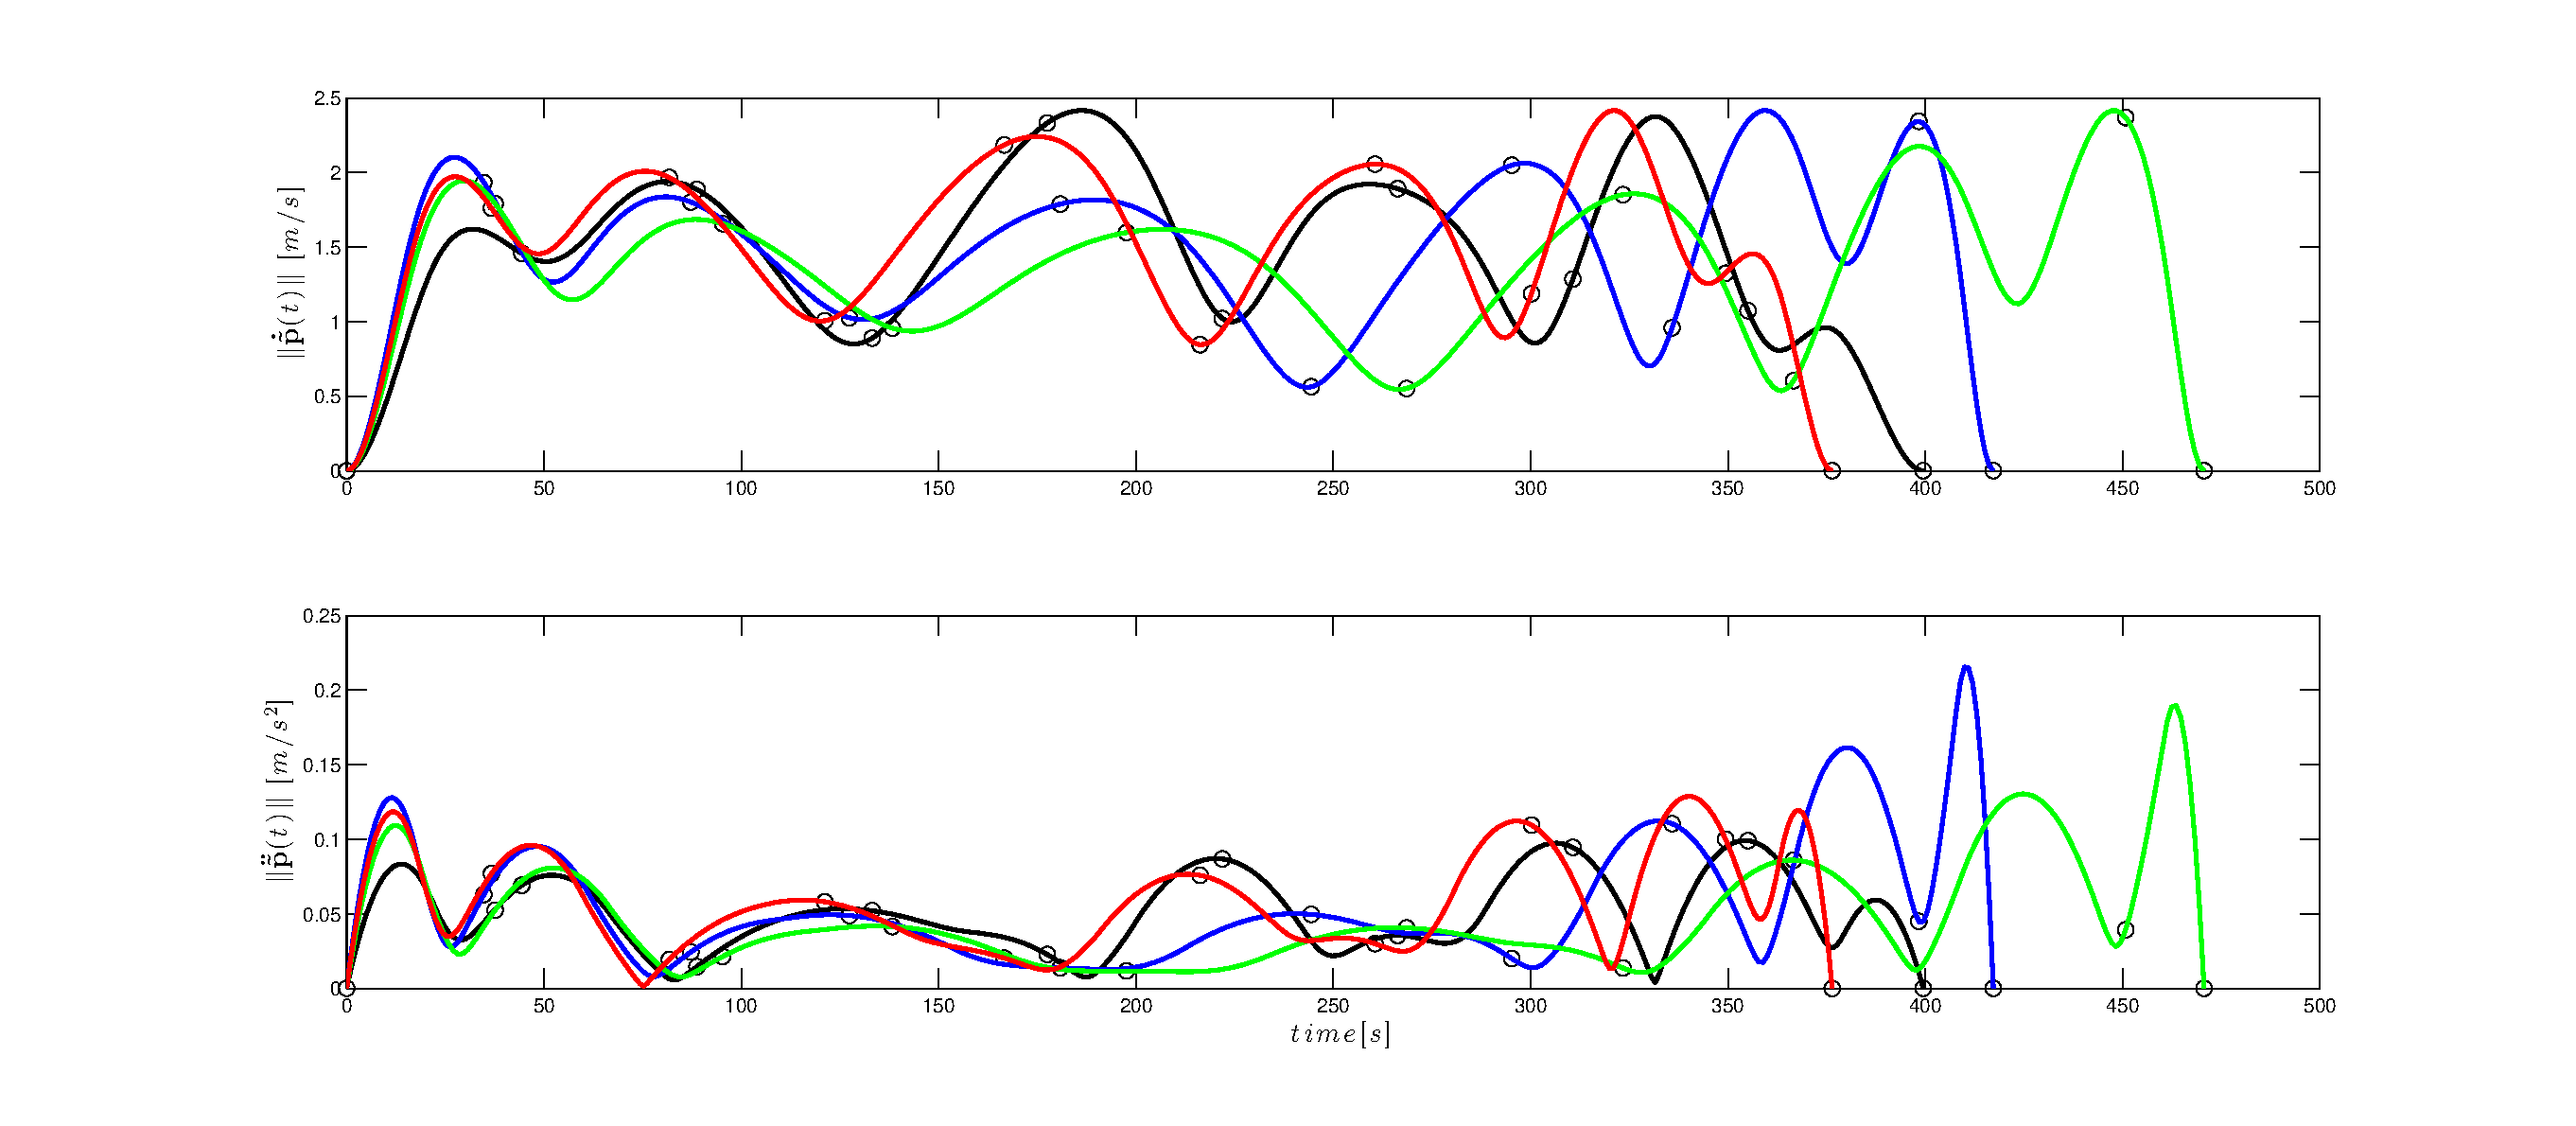
\includegraphics[width = \textwidth]{graphics/Parameterization4_road_vel_acc.eps}
  \end{minipage}
  \caption{Velocity and acceleration of the quartic road trajectory with a motion law which, in this case, limits the maximum velocity. Compare \ref{sec:motionLaw} Uniform:black, Chord length: blue, Arc length: green, Centripetal: red}
  \label{fig:para road vel acc}
\end{figure}

In figure \ref{fig:para road vel acc} the effect of the different distributions on the velocity and acceleration resulting from a constant time scaling can clearly be seen. The chord length as well as the arc length distribution keep the velocity more or less constant but start oscillating at the end of the track.


\subsection{Spline Degree}
{\bf first: explain, show continuity\\
second: Decision with Propulsion Dynamics and oscillation}
\subsubsection{Continuity}
As soon as we talk of splines the question about the spline order arises. Of what degree are the polynomials which make up the spline curve. If polynomials of degree one are used then already the first derivative of the curve will not be continuous anymore. In the case of a trajectory the continuity of the path will directly have an influence on the continuity of the motion as can be seen from the equations \eqref{vel_acc} or in figure \ref{fig:continuity}. So are e.g. cubic splines discontinuous in the jerk whereas quartic is still continuous and quintic splines would be continuous up to the snap. 

\begin{figure}[H]
  \begin{minipage}[t]{0.96\textwidth}
    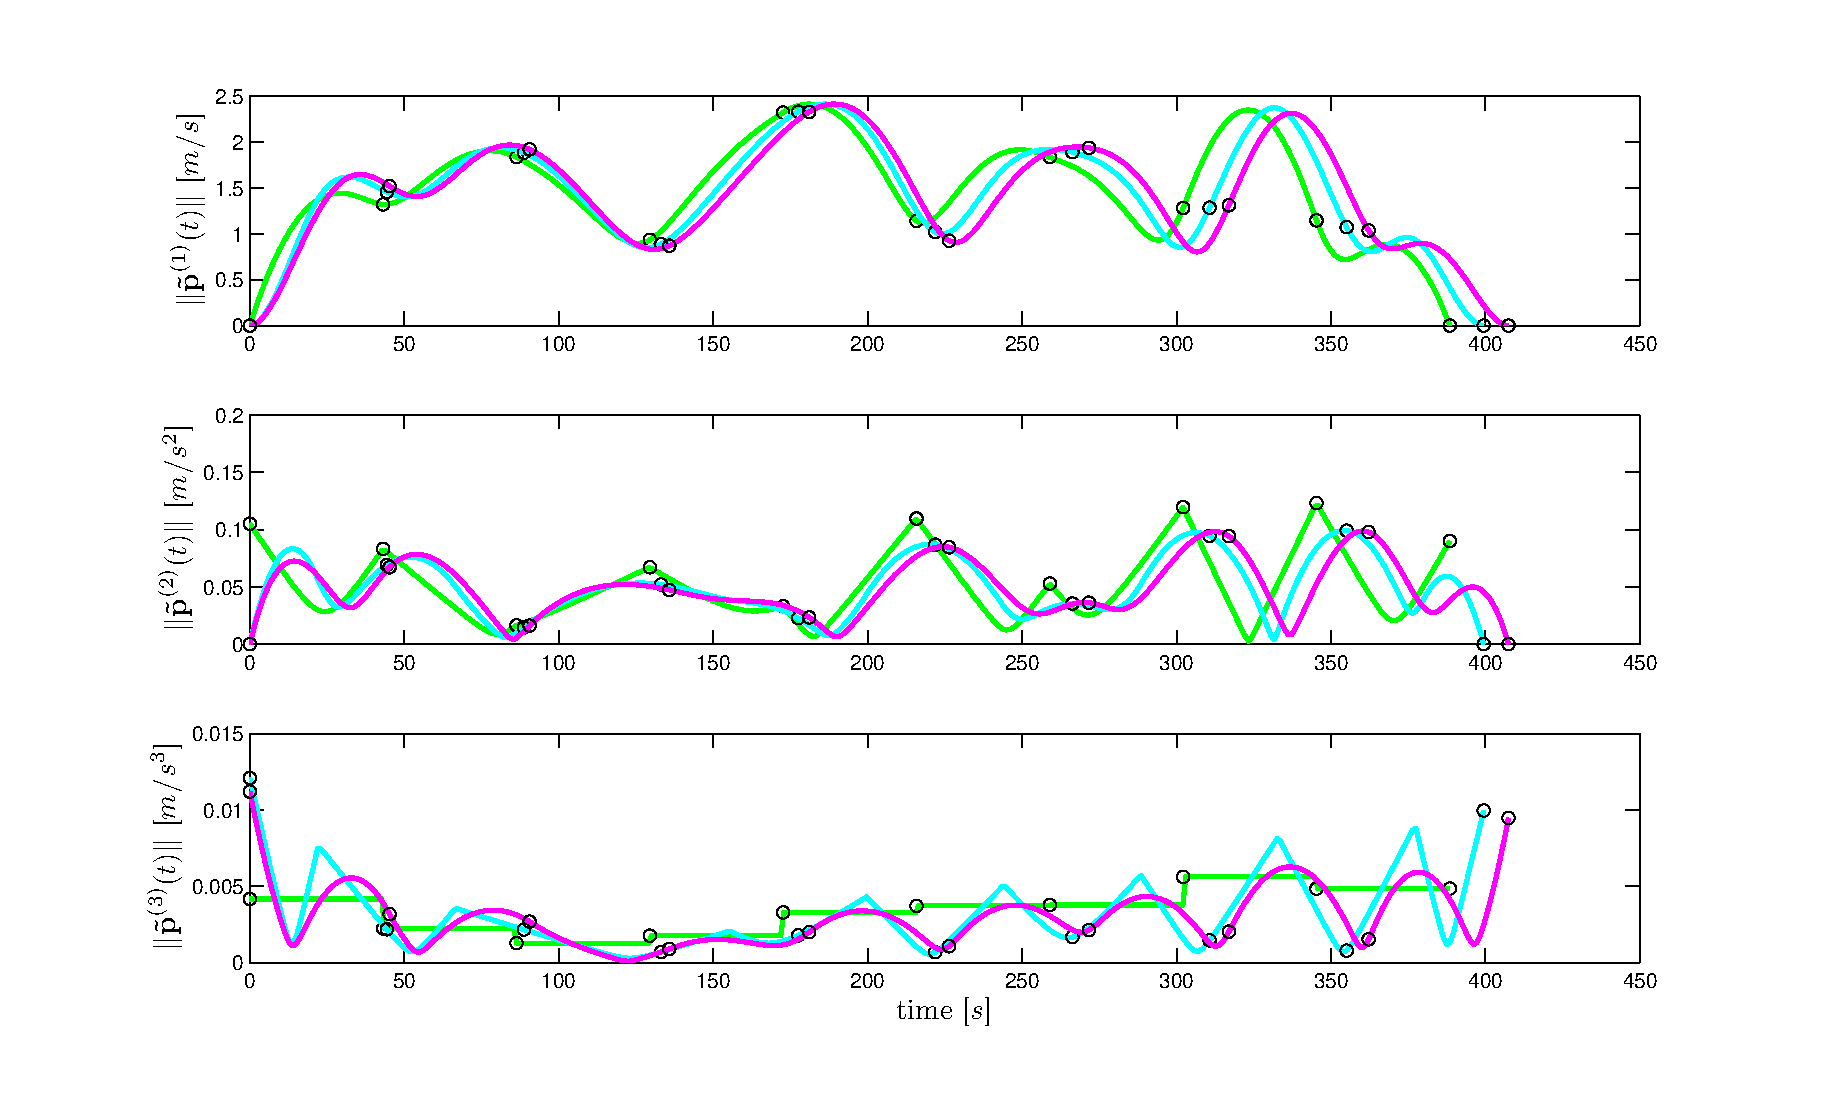
\includegraphics[width = \textwidth]{graphics/continuity.eps}
  \end{minipage}
  \caption{The different degrees of continuity for cubic (green), quartic(blue) and quintic(magenta) splines}
  \label{fig:continuity}
\end{figure}



 For \textsc{Skye} it was intuitively clear that at least cubic splines had to be used. This is due to its propulsion system, which is briefly described in \ref{sec:system overview} and in detail in \cite{schaffnervu}. The orientation of the thrusters cannot be turned immediately. Therefore the trajectory should not ask for a step input for the orientation of thruster which is respected by using cubic splines or splines of higher degree. However in order to find out whether even the dynamics of the thrusters or further dynamics of the positioning motor had to be considered, the whole propulsion system was fed with force calculated from the acceleration $F_x=m_tot*a_x$. As can be seen from figure \ref{forces} the propulsion system is able to handle all resulting inputs of the cubic, quartic and quintic splines.
 
\begin{figure}[H]
  \begin{minipage}[t]{0.96\textwidth}
    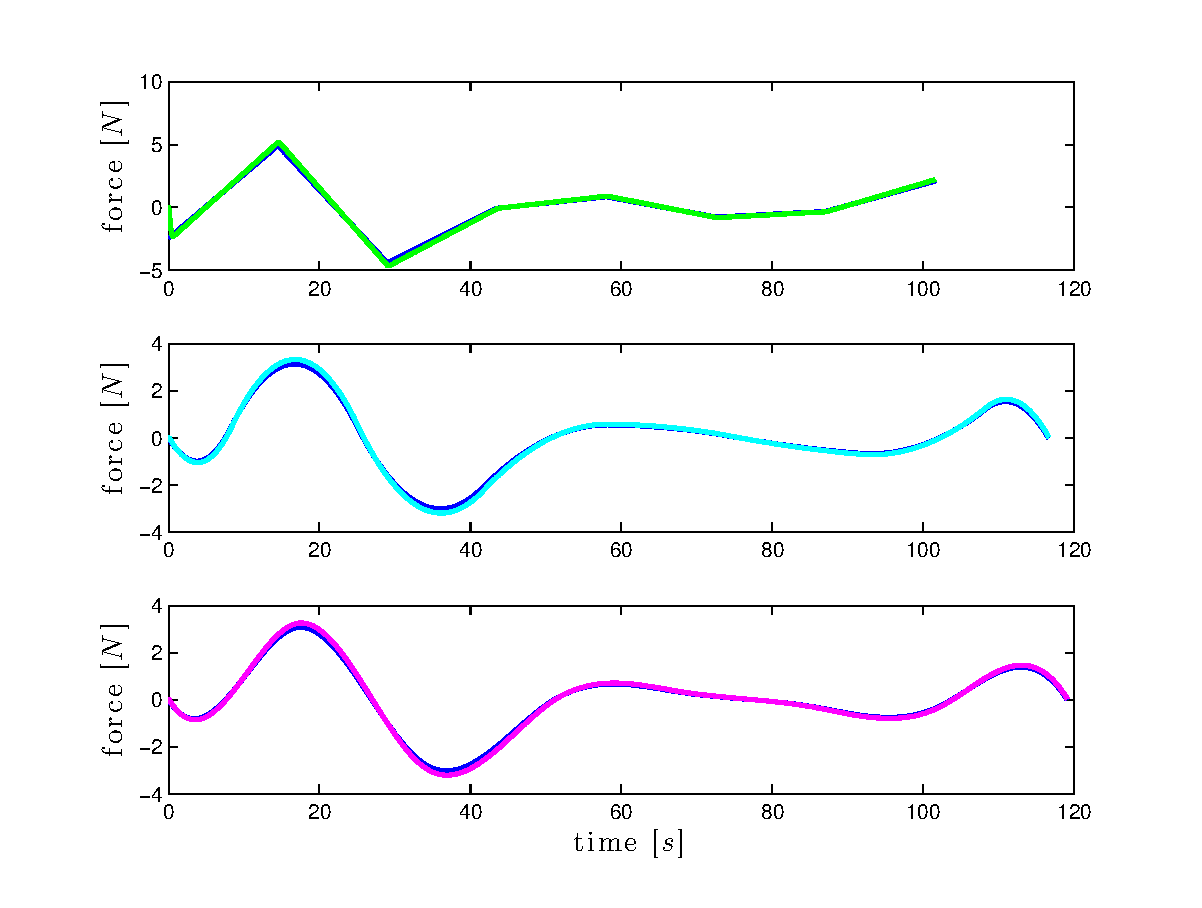
\includegraphics[width = \textwidth]{graphics/forces.eps}
  \end{minipage}
  \caption{The comparison of the forces output of the propulsion dynamics and the forces input resulting from the different degrees of splines; input:blue, output:cubic-green, quartic-blue, quintic-magenta}
\label{fig:forces}
\end{figure} 

The small deviations between the input and the output forces are a result of interpolation, done in the propulsion system \cite{schaffnervu}, and are not a result of an inadequate input. However, BLABLA.....see deviations, but much faster dynamics therefore neglectable.



\subsection{Boundary Conditions}
v0, acc0, vn, accn null, alternative, erstes stueck der kurve durch ein polynom ersetzen.

\subsection{Implementation}


\section{Motion Law}
\label{sec:motionLaw}
\subsection{System Constraints}
\label{subsec:systemConstraints}
In order to plan a feasible trajectory one has to know the capabilities of the system. Here just a basic derivation for the velocities and accelerations is given, for more details refer to (!!!!Bsc Thesis Joe, Bsc Thesis Andy)\\

The maximum feasible acceleration in any direction is calculated to be:

\begin{equation}
  \left|a_{max} \right| =  \frac{\left|F_{res, w}\right|}{m_{tot}} = 0.96 m/s^2
\end{equation}

Whereas the $F_{res,w}$ is the force resulting from all four thrusters operated under full load in the worst direction and $m_{tot}$ is the sum of the masses of the helium, the virtual mass and the mass of the system itself.\\


The maximum feasible velocity in any direction is calculated to be:

\begin{equation}
\left|v_{max} \right| = \sqrt{\frac{\left|F_{res,w} \right|}{\frac{1}{2}c_d \rho \pi r^2}}=2.9 m/s
\end{equation}

which is nothing but $ \left|F_{res,min} \right| = \left|F_{dray} \right| $.\\

For trajectories for position and orientation the maximal feasible angular acceleration is also important. It is calculated to be:

\begin{equation}
  \left|\Psi_{max} \right| =  \frac{\left|M_{res,w}\right|}{\left| \lambda_{max, J_{B}} \right|} = 2.06 rad/s^2 
\end{equation}

which is quite conservative because it is assumed that worst axis for turning is also the principle axis of the inertia tensor with the highest inertia.\\

Since the system is almost undamped for rotations, the rotational velocities will never be the limiting factor.

\subsection{Time Scaling}
\label{subsec:timeScaling}

\section{Controller Implementation}
Some commonly used trajectory controllers\footnote{\cite{snider} provides a good overview to trajectory control.} are tested to follow the defined trajectories. The \textit{Trajectory following} controller supplies the system's position controller \cite{meier} with a feed forward reference signal. Although it delivers good results for ideal case, the tracking get worse for the non perfect model case. The \textit{pure pursuit} controller, which is based on a lookahead point as well as the \textit{cross track error} controller dynamically react on model uncertainties and yield therefore to more robust path tracking results.
\\
BLA BLA introduce notation.. $r(t)$ bla.

 XXXX see \cite{snider} and \cite{deluca}
\label{sec:controllerImplementation}
\subsection{Trajectory Following}
Assuming a perfect model and a trajectory considering all system constraints\footnote{I.e. saturations of $\dot{r}(t)$ and its derivatives.}, the position $r\left(t\right)$ of the system can be assumed to be equal to the trajectory $\tilde{p}(t)$ at any time. Therefore, a straight forward way of a trajectory controller is to follow the trajectory $\tilde{p}(t)$ for every time $t$. This yields to accurate tracking in a safe environment \cite{doesegger}.
\\
A position controller with feedforward terms for velocity and acceleration as described in \cite{meiermueri} can therefore be used with the reference input

\begin{equation}
  [r_{ref}(t), \; \dot{r}_{ref}(t), \; \ddot{r}_{ref}(t)]^T = [\tilde{p}(t), \; \dot{\tilde{p}}(t), \; \ddot{\tilde{p}}(t)]^T
\end{equation}

The controller scheme is shown in figure \ref{fig:trajectoryfollowing}. 

%$\left[ \begin{array}{c} {\bf r}(t) \\ {\bf \dot{r}}(t) \end{array} \right]$
\begin{figure}[h]
    \centering
    \def\svgwidth{0.4\columnwidth}
    \input{graphics/scene_trajectoryFollowing.pdf_tex}
    \caption{For a perfect model and a trajectory ${\bf \tilde{p}}(t)$ considering all system constraints, the position ${\bf{r}}(t)$ will correctly follow the trajectory.}
    \label{fig:scene_trajectoryFollowing}
\end{figure}

\begin{figure}[h]
    \centering
    \def\svgwidth{\columnwidth}
    \input{graphics/controller_trajectoryFollowing.pdf_tex}
    \caption{Trajectory following controller. The value of the parameter $t$ of the trajectory is equal to the current time.}
    \label{fig:trajectoryfollowing}
\end{figure}


Testing the controller yields good performance.. figure \ref{fig:trajFoll_tracking} some BLA BLA



Furthermore, we observed dynamics \ref{fig:trajFoll_dynamics} there are much too many pictures withing the text .. there are much too many pictures withing the text .. there are much too many pictures withing the text .. there are much too many pictures withing the text .. there are much too many pictures withing the text .. there are much too many pictures withing the text .. there are much too many pictures withing the text .. there are much too many pictures withing the text .. there are much too many pictures withing the text .. 


\begin{figure}[h]
    \centering
    \includegraphics[width = \textwidth]{trackings/figure_2D_road_SplineDegree3_trajectoryFollowing_Disturbance_0}
  \hfill
  \caption{BLA dynamics}
  \label{fig:trajFoll_dynamics}
\end{figure}

It is definitively too much to show figure \ref{fig:trajFoll_sysConstraints} and it has to be improved by showing both trajectory and trace.. there are much too many pictures withing the text .. there are much too many pictures withing the text .. there are much too many pictures withing the text .. there are much too many pictures withing the text .. \\ there are much too many pictures withing the text .. there are much too many pictures withing the text .. there are much too many pictures withing the text .. there are much too many pictures withing the text .. 

%\begin{figure}[h]
%    \centering
%    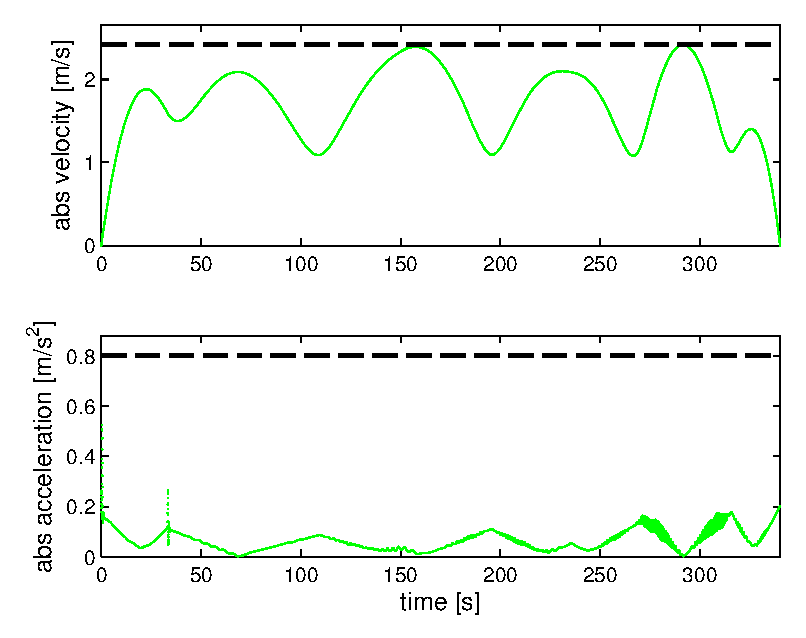
\includegraphics[width = 0.8\textwidth]{trackings/figure_1D_road_SplineDegree3_trajectoryFollowing_Disturbance_0}
%  \hfill
%  \caption{BLA dynamics}
%  \label{fig:trajFoll_dynamics}
%\end{figure}





The results before were all by perfect models. Now with distrubances..there are much too many pictures withing the text .. there are much too many pictures withing the text .. there are much too many pictures withing the text .. there are much too many pictures withing the text .. there are much too many pictures withing the text .. there are much too many pictures withing the text .. there are much too many pictures withing the text .. there are much too many pictures withing the text .. there are much too many pictures withing the text .. there are much too many pictures withing the text .. there are much too many pictures withing the text .. there are much too many pictures withing the text .. 

%\begin{figure}[H]
%  \begin{minipage}[t]{0.32\textwidth}
%    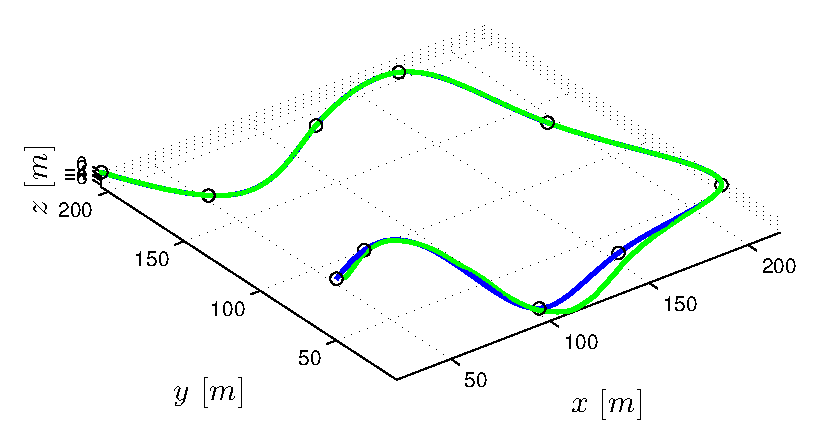
\includegraphics[width = \textwidth]{trackings/figure_3D_road_SplineDegree3_trajectoryFollowing_Disturbance_1}
%  \end{minipage}
%  \hfill
%  \begin{minipage}[t]{0.32\textwidth}
%    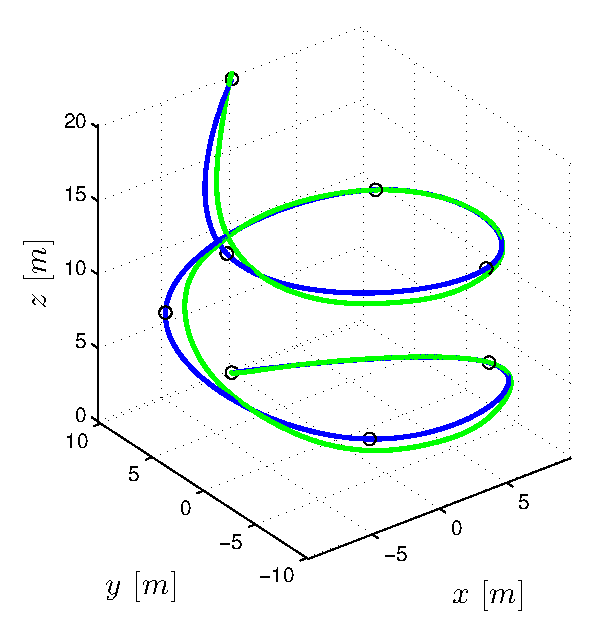
\includegraphics[width = \textwidth]{trackings/figure_3D_helix_SplineDegree3_trajectoryFollowing_Disturbance_1}
%  \end{minipage}
%  \hfill
%  \begin{minipage}[t]{0.32\textwidth}
%    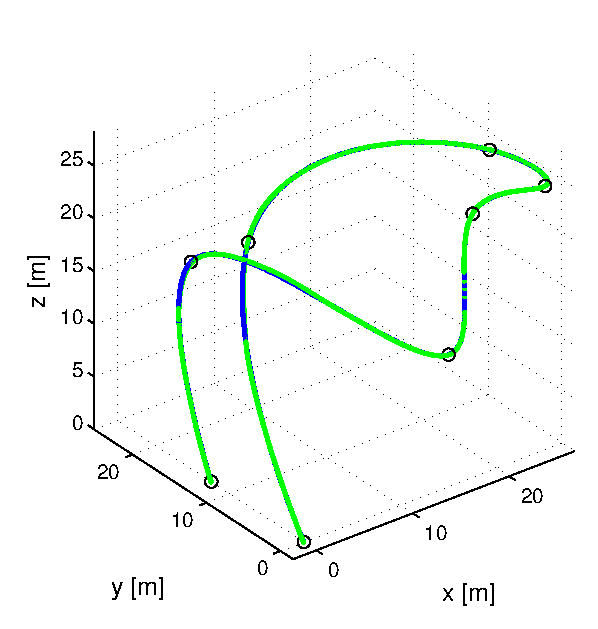
\includegraphics[width = \textwidth]{trackings/figure_3D_agile_SplineDegree3_trajectoryFollowing_Disturbance_1}
%  \end{minipage}
%  \caption{BLA tracking but this time with wind}
%  \label{fig:trajFollWind_tracking}
%\end{figure}


\subsection{Pure Pursuit Controller}
Another commonly used controller to track paths is Pure Pursuit \cite{snider}. To consider all dynamics of the trajectory, the reference intput is based on a lookahead point $\tilde{p}(t_{cl}+\Delta T) = {\bf \tilde{p}}(t_{cl}) + \Delta T \cdot {\bf\dot{ \tilde{p}}}(t_{cl}) + \frac{1}{2} \Delta T^2 \cdot {\bf\ddot{ \tilde{p}}}(t_{cl}) + \mathcal{O}(\Delta T^3)$ that considers terms of ${\bf \tilde{p}}(t)$ and all its derivatives\footnote{Note, that this is a simple and robust alternative to any derivative controller.}.

%$ {\bf \dot{r}}_{ref}(t) $
\begin{figure}[h]
    \centering
    \def\svgwidth{0.5\columnwidth}
    \input{graphics/scene_purePursuit.pdf_tex}
    \caption{Pure pursuit yields to extremly awesome tracking.}
    \label{fig:scene_purePursuit}
\end{figure}

\begin{figure}[h]
    \centering
    \def\svgwidth{\columnwidth}
    \input{graphics/controller_purePursuit.pdf_tex}
    \caption{Pure pursuit yields to extremly awesome tracking.}
    \label{fig:purePursuit}
\end{figure}

And here again, the resulting trajectories altough they look the same as in the subsection before.

%\begin{figure}[H]
%  \begin{minipage}[t]{0.32\textwidth}
%    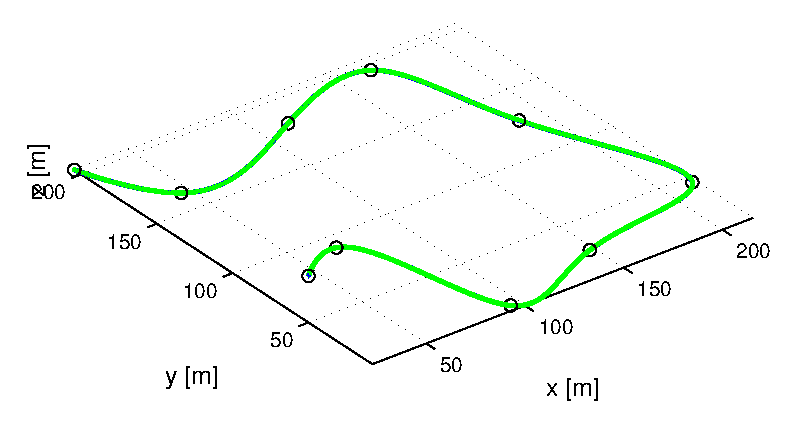
\includegraphics[width = \textwidth]{trackings/figure_3D_road_SplineDegree3_purePursuit_Disturbance_0}
%  \end{minipage}
%  \hfill
%  \begin{minipage}[t]{0.32\textwidth}
%    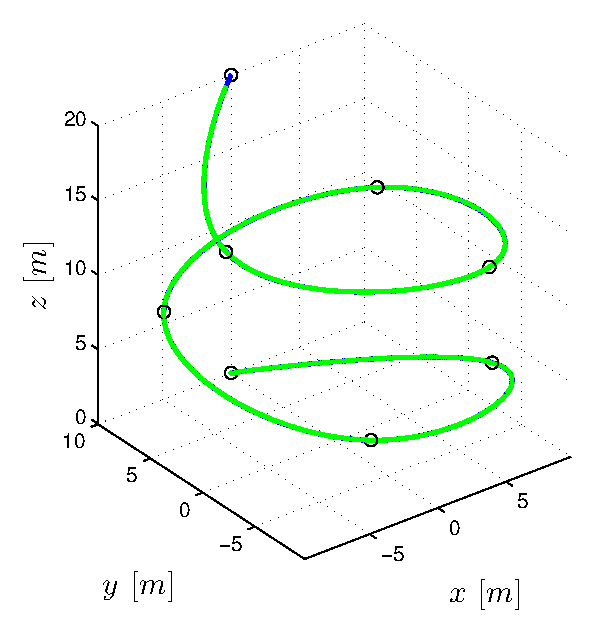
\includegraphics[width = \textwidth]{trackings/figure_3D_helix_SplineDegree3_purePursuit_Disturbance_0}
%  \end{minipage}
%  \hfill
%  \begin{minipage}[t]{0.32\textwidth}
%    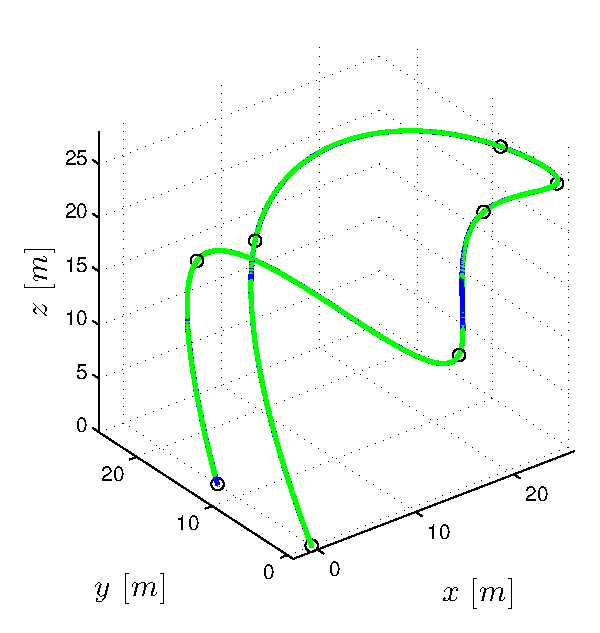
\includegraphics[width = \textwidth]{trackings/figure_3D_agile_SplineDegree3_purePursuit_Disturbance_0}
%  \end{minipage}
%  \caption{BLA pure pursuit}
%  \label{fig:purePursuit_tracking}
%\end{figure}
%
%\begin{figure}[H]
%  \begin{minipage}[t]{0.32\textwidth}
%    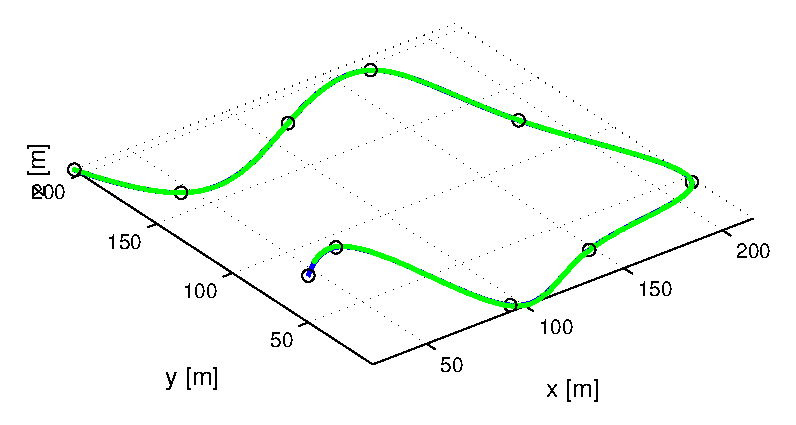
\includegraphics[width = \textwidth]{trackings/figure_3D_road_SplineDegree3_purePursuit_Disturbance_1}
%  \end{minipage}
%  \hfill
%  \begin{minipage}[t]{0.32\textwidth}
%    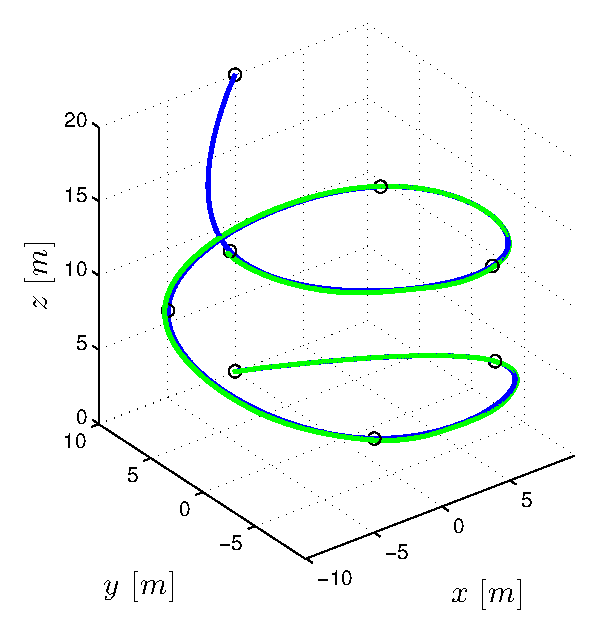
\includegraphics[width = \textwidth]{trackings/figure_3D_helix_SplineDegree3_purePursuit_Disturbance_1}
%  \end{minipage}
%  \hfill
%  \begin{minipage}[t]{0.32\textwidth}
%    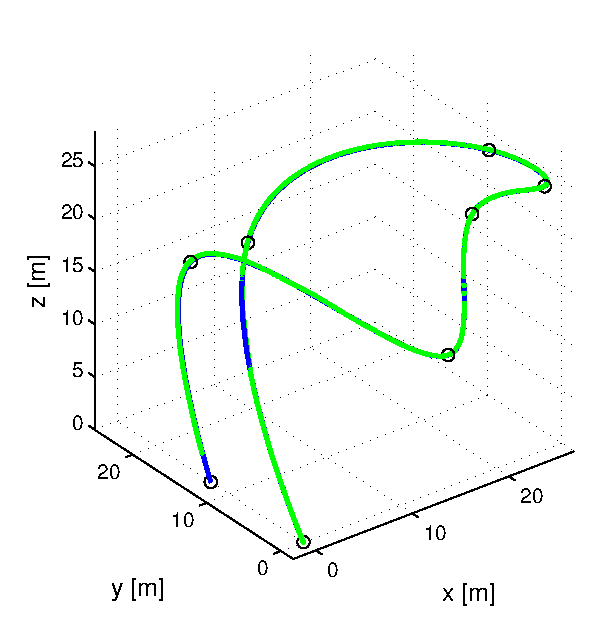
\includegraphics[width = \textwidth]{trackings/figure_3D_agile_SplineDegree3_purePursuit_Disturbance_1}
%  \end{minipage}
%  \caption{BLA pure pursuit and here with wind}
%  \label{fig:purePursuit_tracking}
%\end{figure}




\subsection{Cross Track Error Controller}
see \cite{williams}

%$\left[ \begin{array}{c} {\bf \tilde{p}}(t) \\ {\bf \dot{\tilde{p}}}(t) \\ {\bf \ddot{\tilde{p}}}(t) \end{array} \right]$
\begin{figure}[h]
    \centering
    \def\svgwidth{0.5\columnwidth}
    \input{graphics/scene_crossTrack.pdf_tex}
    \caption{Cross Track Error Control yields to extremly awesome tracking.}
    \label{fig:scene_crossTrack}
\end{figure}


\begin{figure}[h]
    \centering
    \def\svgwidth{\columnwidth}
    \input{graphics/controller_crossTrack.pdf_tex}
    \caption{Cross Track Error Control yields to extremly awesome tracking.}
    \label{fig:crossTrack}
\end{figure}


%\begin{figure}[H]
%  \begin{minipage}[t]{0.32\textwidth}
%    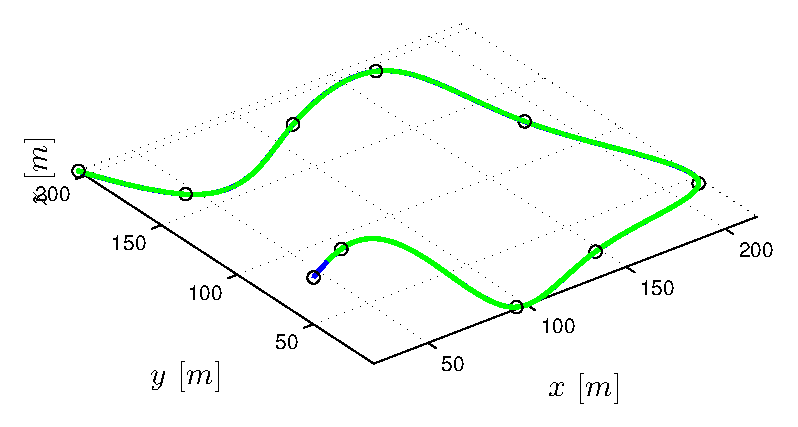
\includegraphics[width = \textwidth]{trackings/figure_3D_road_SplineDegree3_crossTrack_Disturbance_0}
%  \end{minipage}
%  \hfill
%  \begin{minipage}[t]{0.32\textwidth}
%    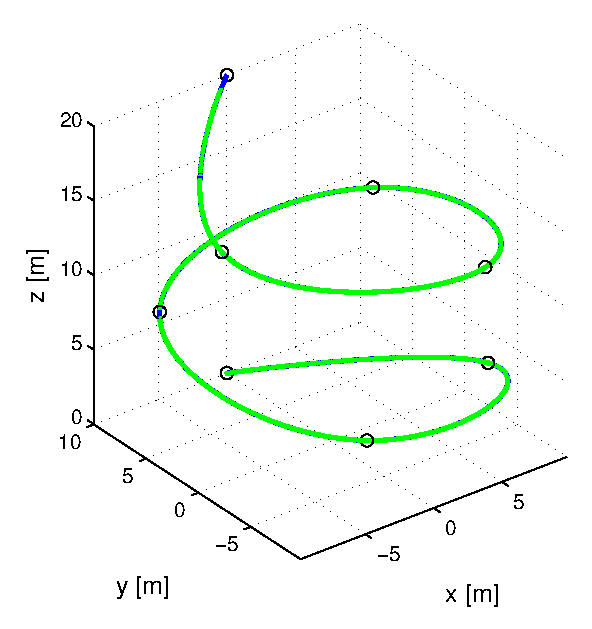
\includegraphics[width = \textwidth]{trackings/figure_3D_helix_SplineDegree3_crossTrack_Disturbance_0}
%  \end{minipage}
%  \hfill
%  \begin{minipage}[t]{0.32\textwidth}
%    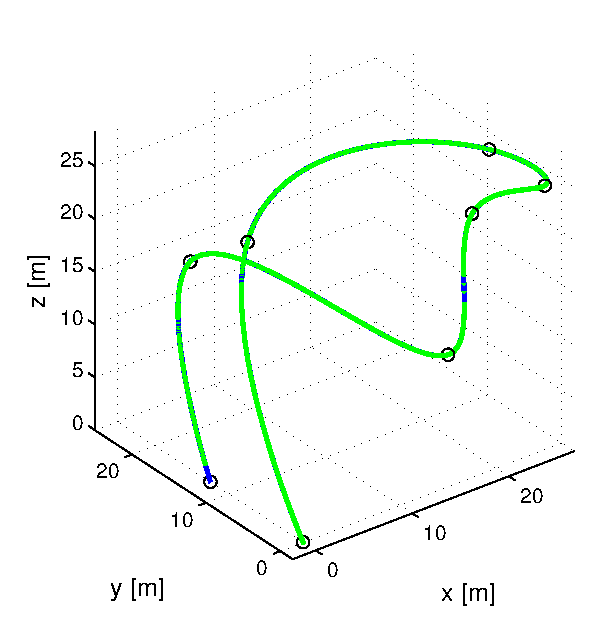
\includegraphics[width = \textwidth]{trackings/figure_3D_agile_SplineDegree3_crossTrack_Disturbance_0}
%  \end{minipage}
%  \caption{BLA cross track}
%  \label{fig:crossTrack_tracking}
%\end{figure}
%
%\begin{figure}[H]
%  \begin{minipage}[t]{0.32\textwidth}
%    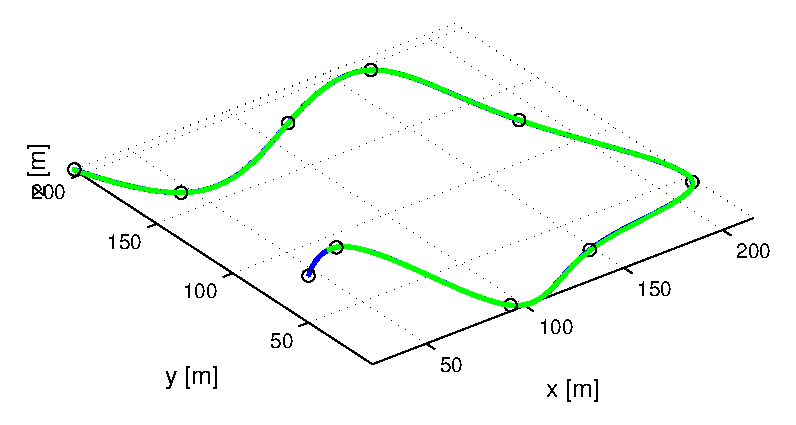
\includegraphics[width = \textwidth]{trackings/figure_3D_road_SplineDegree3_crossTrack_Disturbance_1}
%  \end{minipage}
%  \hfill
%  \begin{minipage}[t]{0.32\textwidth}
%    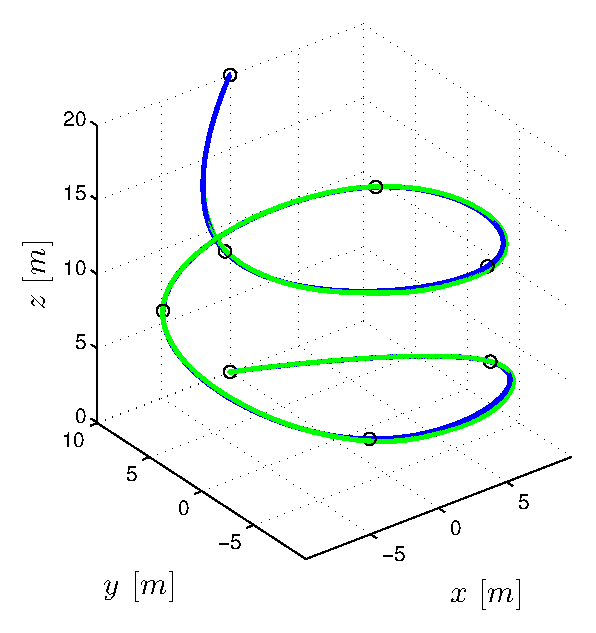
\includegraphics[width = \textwidth]{trackings/figure_3D_helix_SplineDegree3_crossTrack_Disturbance_1}
%  \end{minipage}
%  \hfill
%  \begin{minipage}[t]{0.32\textwidth}
%    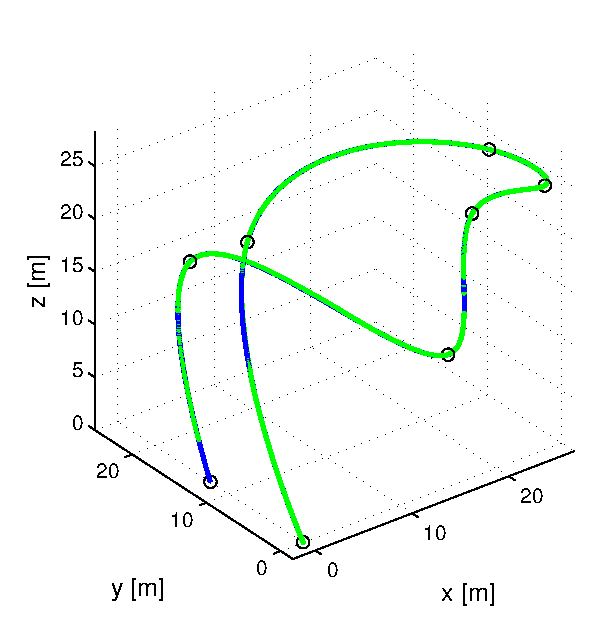
\includegraphics[width = \textwidth]{trackings/figure_3D_agile_SplineDegree3_crossTrack_Disturbance_1}
%  \end{minipage}
%  \caption{BLA cross track with wind}
%  \label{fig:crossTrackWind_tracking}
%\end{figure}

\section{Results}
\label{sec:results}

\paragraph{Perfect Model OR IDEAL CASE}
\label{par:results_perfect_model}

\begin{figure}[h]
  \begin{minipage}[t]{0.32\textwidth}
    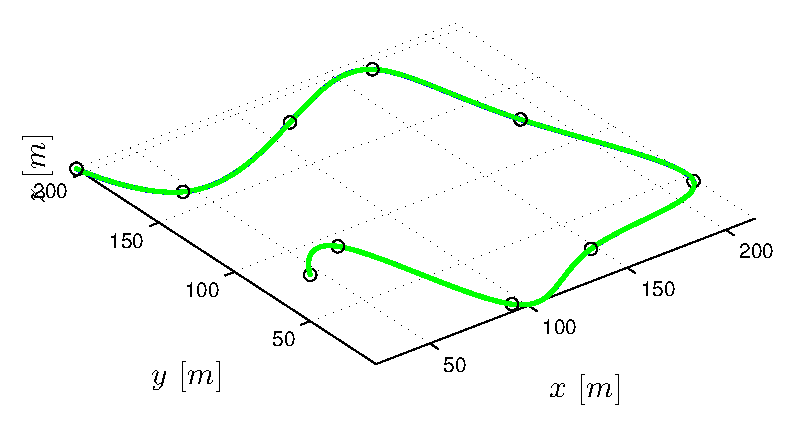
\includegraphics[width = \textwidth]{trackings/figure_3D_road_SplineDegree3_trajectoryFollowing_Disturbance_0}
  \end{minipage}
  \hfill
  \begin{minipage}[t]{0.32\textwidth}
    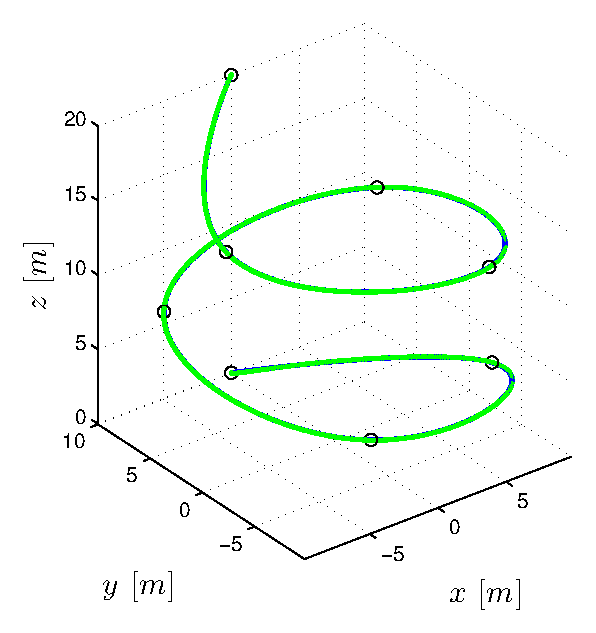
\includegraphics[width = \textwidth]{trackings/figure_3D_helix_SplineDegree3_trajectoryFollowing_Disturbance_0}
  \end{minipage}
  \hfill
  \begin{minipage}[t]{0.32\textwidth}
    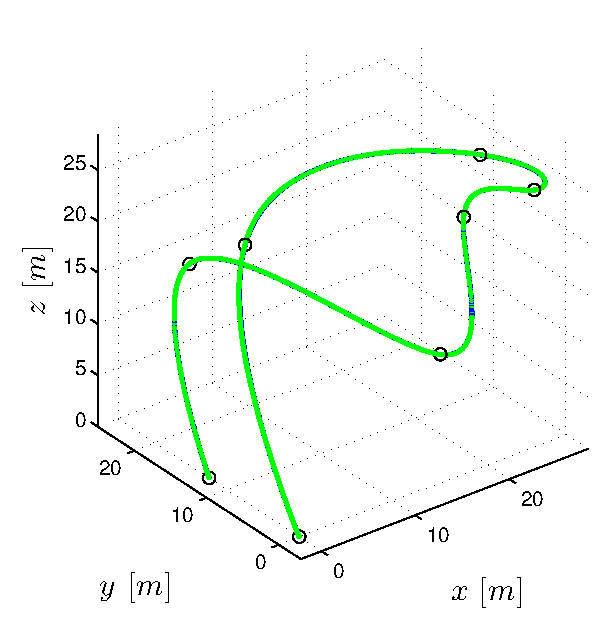
\includegraphics[width = \textwidth]{trackings/figure_3D_agile_SplineDegree3_trajectoryFollowing_Disturbance_0}
  \end{minipage}
  %\caption{BLA tracking }
  \vspace{5pt}
  \begin{minipage}[t]{0.32\textwidth}
    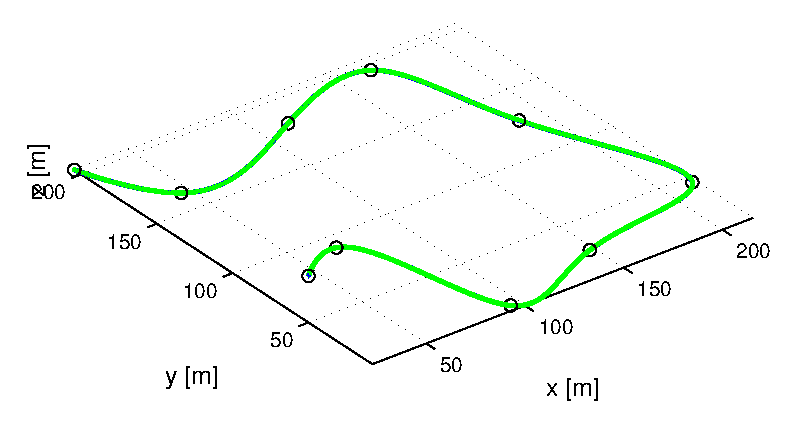
\includegraphics[width = \textwidth]{trackings/figure_3D_road_SplineDegree3_purePursuit_Disturbance_0}
  \end{minipage}
  \hfill
  \begin{minipage}[t]{0.32\textwidth}
    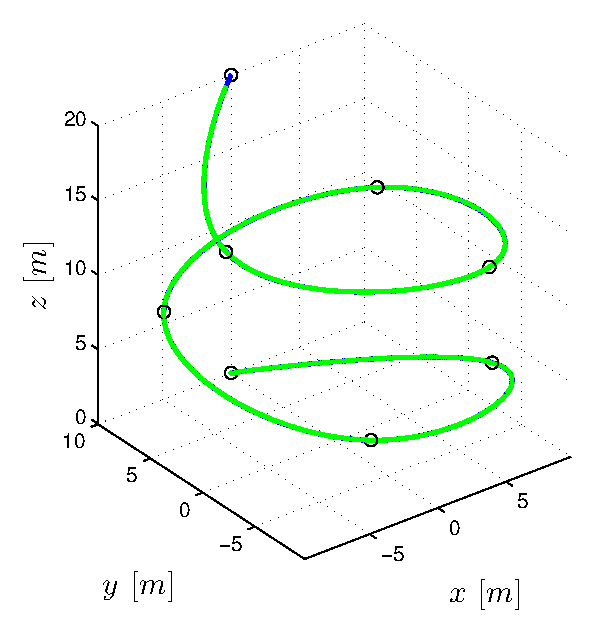
\includegraphics[width = \textwidth]{trackings/figure_3D_helix_SplineDegree3_purePursuit_Disturbance_0}
  \end{minipage}
  \hfill
  \begin{minipage}[t]{0.32\textwidth}
    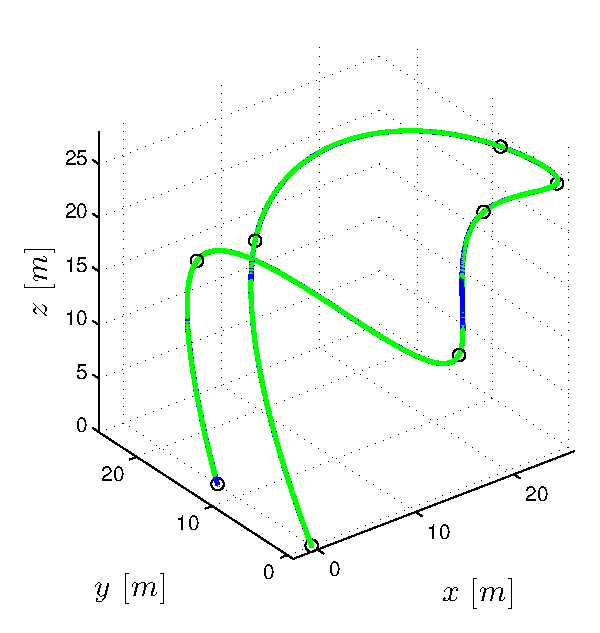
\includegraphics[width = \textwidth]{trackings/figure_3D_agile_SplineDegree3_purePursuit_Disturbance_0}
  \end{minipage}
  %\caption{BLA tracking }
  \vspace{5pt}
  \begin{minipage}[t]{0.32\textwidth}
    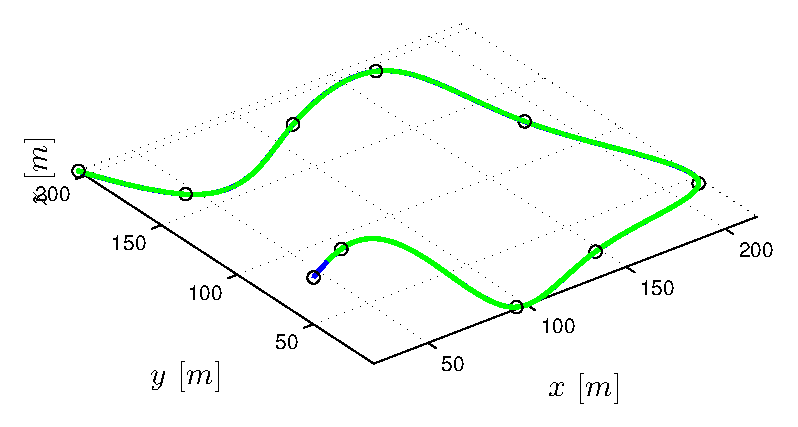
\includegraphics[width = \textwidth]{trackings/figure_3D_road_SplineDegree3_crossTrack_Disturbance_0}
  \end{minipage}
  \hfill
  \begin{minipage}[t]{0.32\textwidth}
    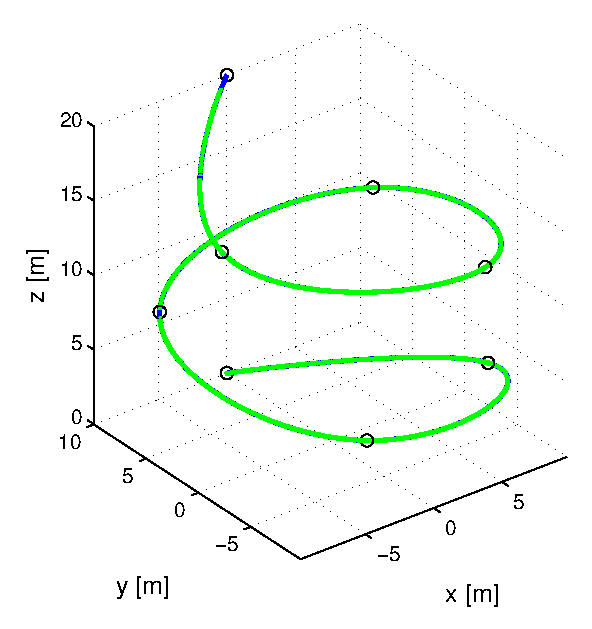
\includegraphics[width = \textwidth]{trackings/figure_3D_helix_SplineDegree3_crossTrack_Disturbance_0}
  \end{minipage}
  \hfill
  \begin{minipage}[t]{0.32\textwidth}
    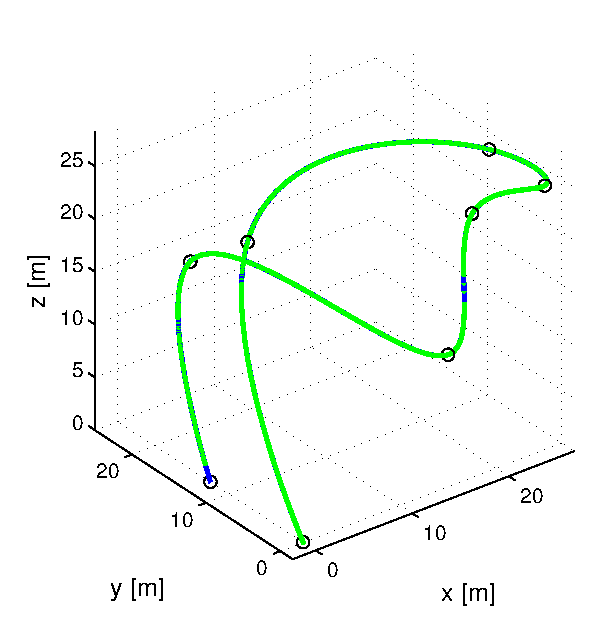
\includegraphics[width = \textwidth]{trackings/figure_3D_agile_SplineDegree3_crossTrack_Disturbance_0}
  \end{minipage}
  \caption{BLA tracking }
  \label{fig:results_perfect_model}
\end{figure}

We can show the results in a table, or we can put it all to the appendix..

\begin{table}[h]
\begin{center}
 \begin{tabular}{lll|lll}
 \hline
 Controller &   & unit & \textit{Road} & \textit{Helix} & \textit{Agile} \\ \hline \hline
 Trajectory Following & Av. Dev. & $[m]$ & 0.007 & 0.017 & 0.014 \\
 Pure Pursuit         & Av. Dev & $[m]$ & 0.007 & 0.009 & 0.017 \\
 Cross Track          & Av. Dev & $[m]$ &  0.007 & 0.007 & 0.006 \\
    
 Trajectory Following & Av. Acc & $[m/s^2]$ & 0.029 & 0.174 & 0.137 \\
 Pure Pursuit         & Av. Acc & $[m/s^2]$ & 0.031 & 0.159 & 0.128 \\
 Cross Track          & Av. Acc & $[m/s^2]$ & 0.029 & 0.159 & 0.126 \\
 \hline
 \end{tabular}
 \caption{Here some absolute results to perfect model estimation.}\vspace{1ex}
 \label{tab:results_perfect_model}
\end{center}
\end{table}

\paragraph{Wind Disturbance}
\label{par:results_wind_disturbance}

\begin{figure}[h]
  \begin{minipage}[t]{0.32\textwidth}
    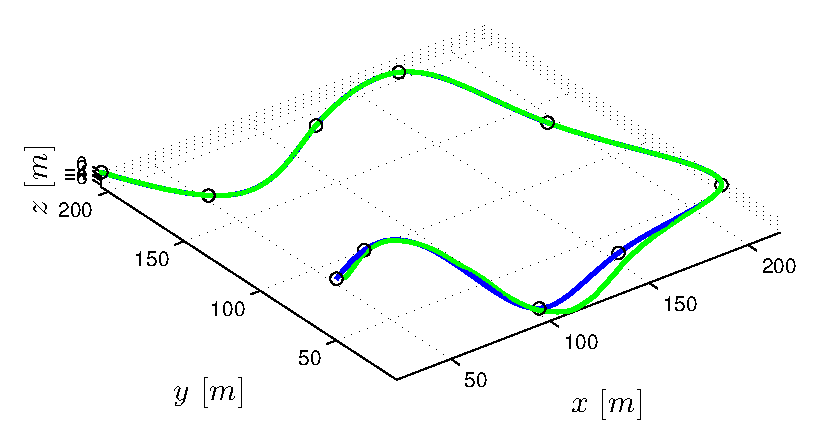
\includegraphics[width = \textwidth]{trackings/figure_3D_road_SplineDegree3_trajectoryFollowing_Disturbance_1}
  \end{minipage}
  \hfill
  \begin{minipage}[t]{0.32\textwidth}
    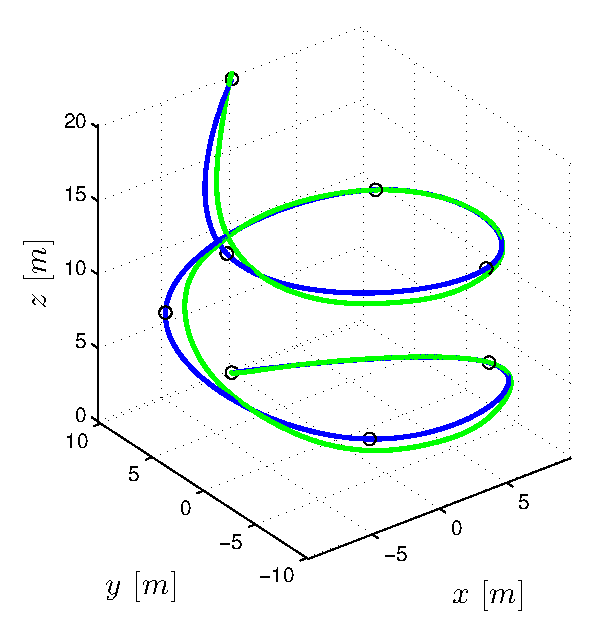
\includegraphics[width = \textwidth]{trackings/figure_3D_helix_SplineDegree3_trajectoryFollowing_Disturbance_1}
  \end{minipage}
  \hfill
  \begin{minipage}[t]{0.32\textwidth}
    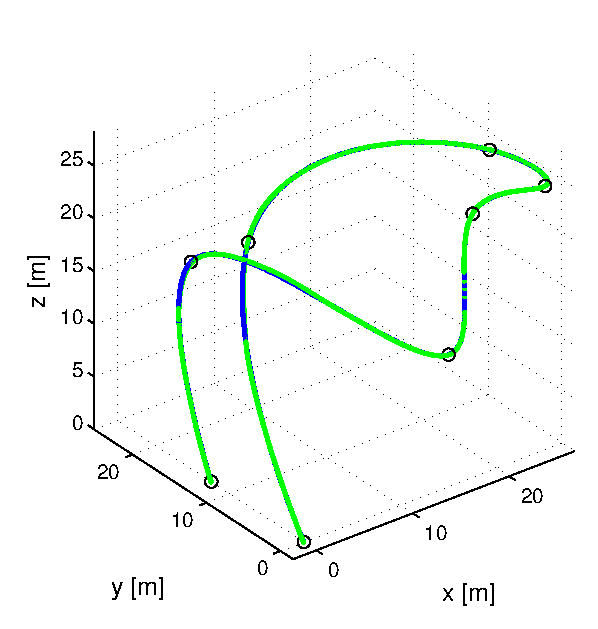
\includegraphics[width = \textwidth]{trackings/figure_3D_agile_SplineDegree3_trajectoryFollowing_Disturbance_1}
  \end{minipage}
  %\caption{BLA tracking }
  \vspace{5pt}
  \begin{minipage}[t]{0.32\textwidth}
    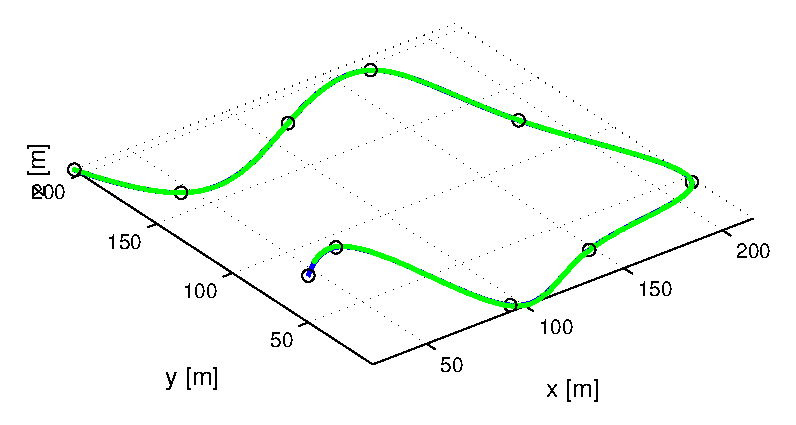
\includegraphics[width = \textwidth]{trackings/figure_3D_road_SplineDegree3_purePursuit_Disturbance_1}
  \end{minipage}
  \hfill
  \begin{minipage}[t]{0.32\textwidth}
    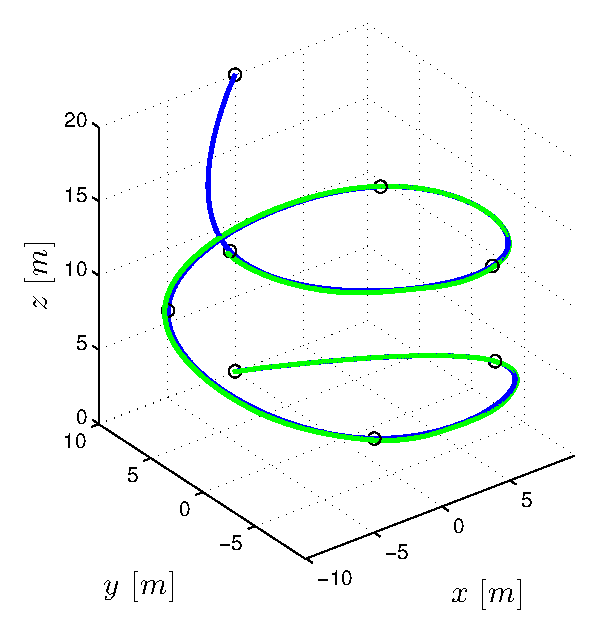
\includegraphics[width = \textwidth]{trackings/figure_3D_helix_SplineDegree3_purePursuit_Disturbance_1}
  \end{minipage}
  \hfill
  \begin{minipage}[t]{0.32\textwidth}
    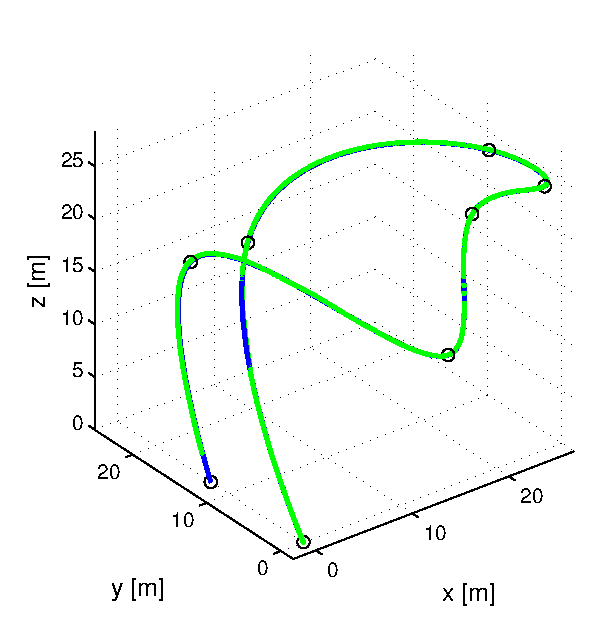
\includegraphics[width = \textwidth]{trackings/figure_3D_agile_SplineDegree3_purePursuit_Disturbance_1}
  \end{minipage}
  %\caption{BLA tracking }
  \vspace{5pt}
  \begin{minipage}[t]{0.32\textwidth}
    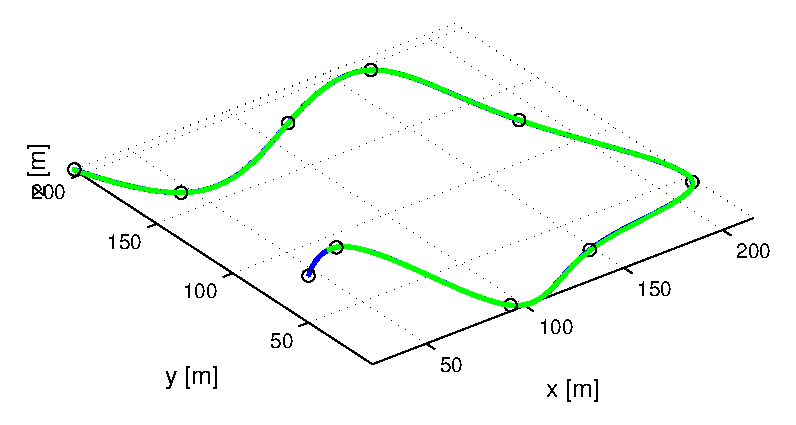
\includegraphics[width = \textwidth]{trackings/figure_3D_road_SplineDegree3_crossTrack_Disturbance_1}
  \end{minipage}
  \hfill
  \begin{minipage}[t]{0.32\textwidth}
    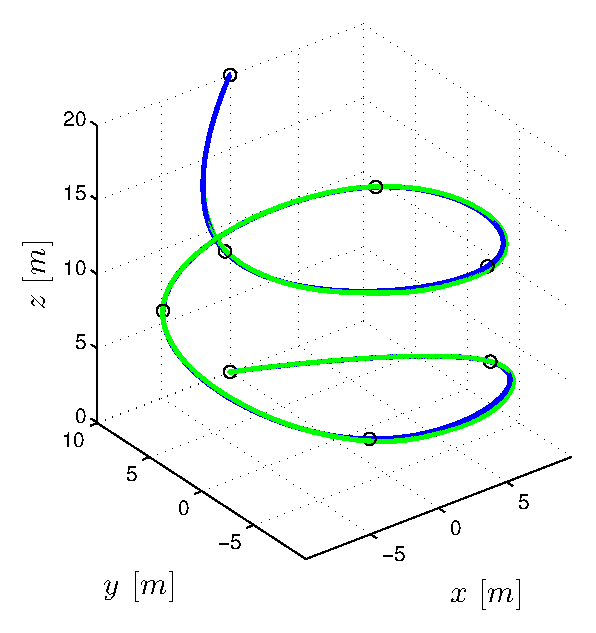
\includegraphics[width = \textwidth]{trackings/figure_3D_helix_SplineDegree3_crossTrack_Disturbance_1}
  \end{minipage}
  \hfill
  \begin{minipage}[t]{0.32\textwidth}
    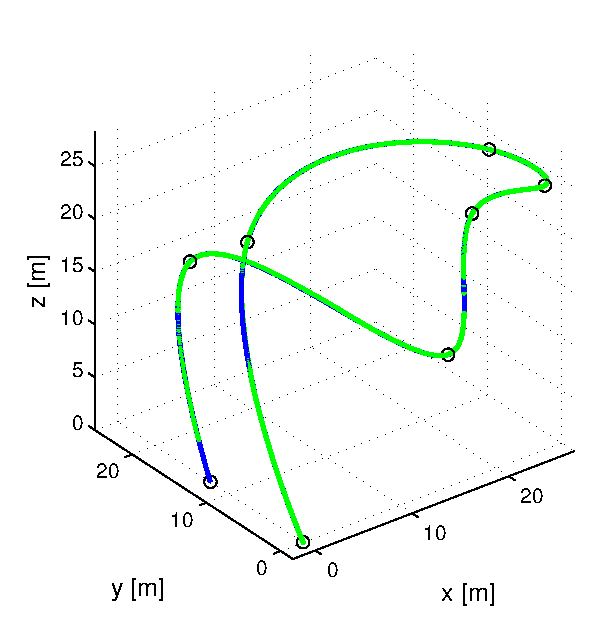
\includegraphics[width = \textwidth]{trackings/figure_3D_agile_SplineDegree3_crossTrack_Disturbance_1}
  \end{minipage}
  \caption{BLA tracking }
  \label{fig:results_wind_disturbance}
\end{figure}

We can show the results in a table, or we can put it all to the appendix..

\begin{table}[h]
\begin{center}
 \begin{tabular}{lll|lll}
 \hline
 Controller &   & unit & \textit{Road} & \textit{Helix} & \textit{Agile} \\ \hline \hline
 Trajectory Following & Av. Dev. & $[m]$ & 1.783 & 0.606 & 0.111 \\
 Pure Pursuit         & Av. Dev & $[m]$ & 0.0785 & 0.098 & 0.037 \\
 Cross Track          & Av. Dev & $[m]$ &  0.034 & 0.061 & 0.023 \\
    
 Trajectory Following & Av. Acc & $[m/s^2]$ & 0.031 & 0.191 & 0.138 \\
 Pure Pursuit         & Av. Acc & $[m/s^2]$ & 0.031 & 0.136 & 0.121 \\
 Cross Track          & Av. Acc & $[m/s^2]$ & 0.028 & 0.140 & 0.120 \\
 \hline
 \end{tabular}
 \caption{Here some absolute results with wind disturbance.}\vspace{1px}
 \label{tab:results_model_uncertainties}
\end{center}
\end{table}

\paragraph{Model Uncertainties}
\label{par:results_model_uncertainties}

\begin{figure}[h]
  \begin{minipage}[t]{0.32\textwidth}
    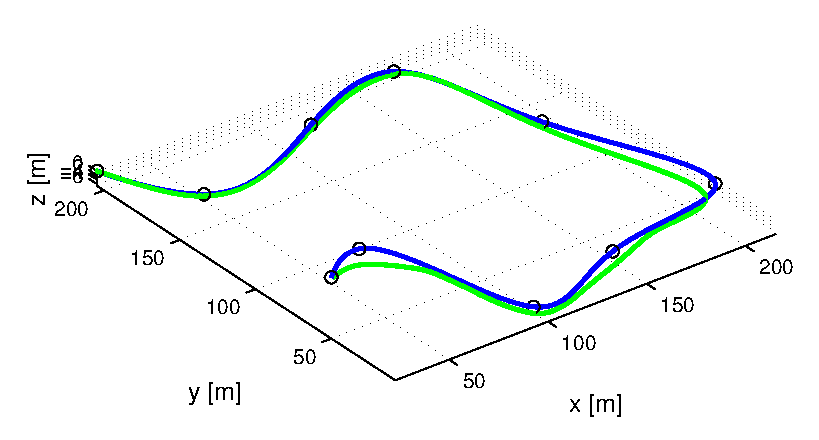
\includegraphics[width = \textwidth]{trackings_wc/figure_3D_road_SplineDegree3_trajectoryFollowing_Disturbance_0}
  \end{minipage}
  \hfill
  \begin{minipage}[t]{0.32\textwidth}
    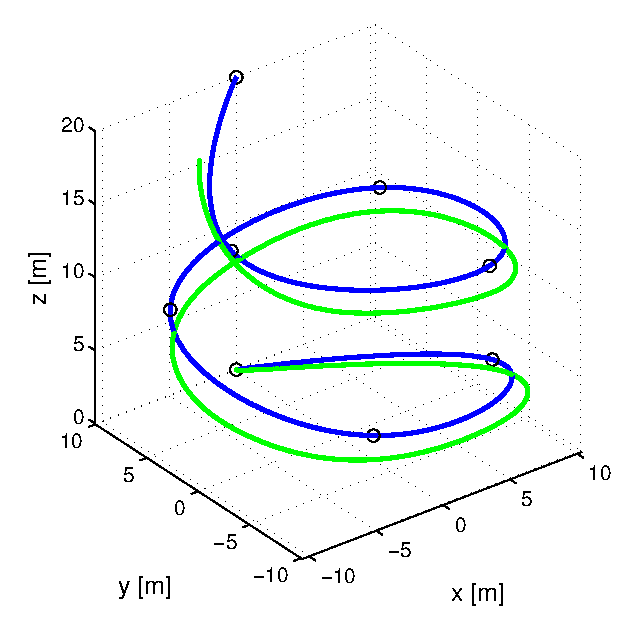
\includegraphics[width = \textwidth]{trackings_wc/figure_3D_helix_SplineDegree3_trajectoryFollowing_Disturbance_0}
  \end{minipage}
  \hfill
  \begin{minipage}[t]{0.32\textwidth}
    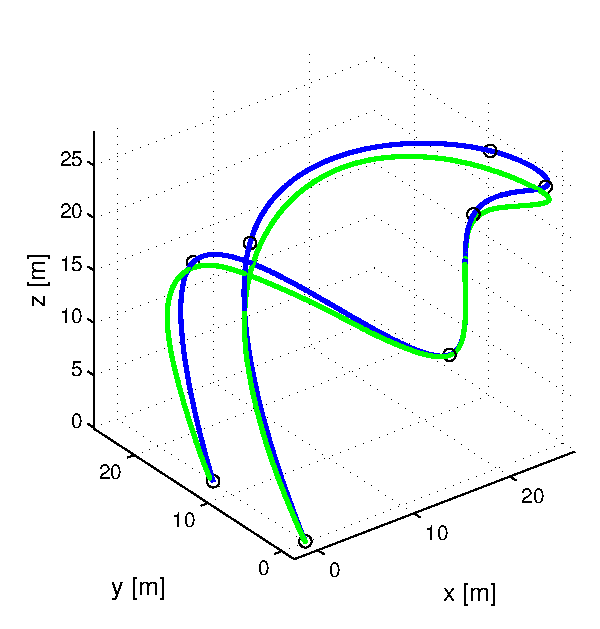
\includegraphics[width = \textwidth]{trackings_wc/figure_3D_agile_SplineDegree3_trajectoryFollowing_Disturbance_0}
  \end{minipage}
  %\caption{BLA tracking }
  \vspace{5pt}
  \begin{minipage}[t]{0.32\textwidth}
    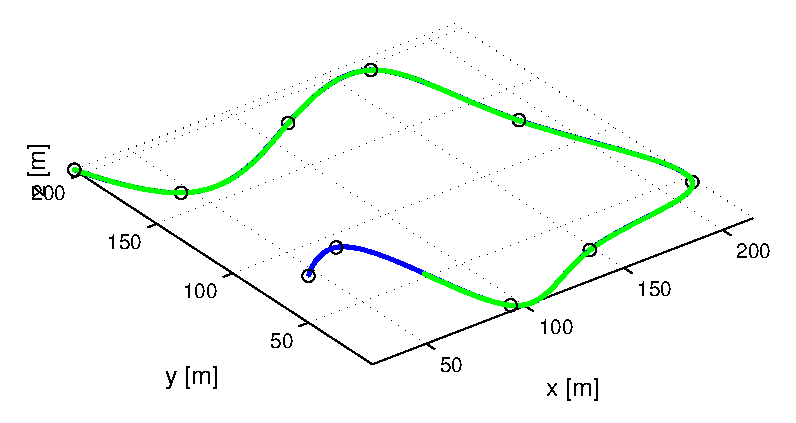
\includegraphics[width = \textwidth]{trackings_wc/figure_3D_road_SplineDegree3_purePursuit_Disturbance_0}
  \end{minipage}
  \hfill
  \begin{minipage}[t]{0.32\textwidth}
    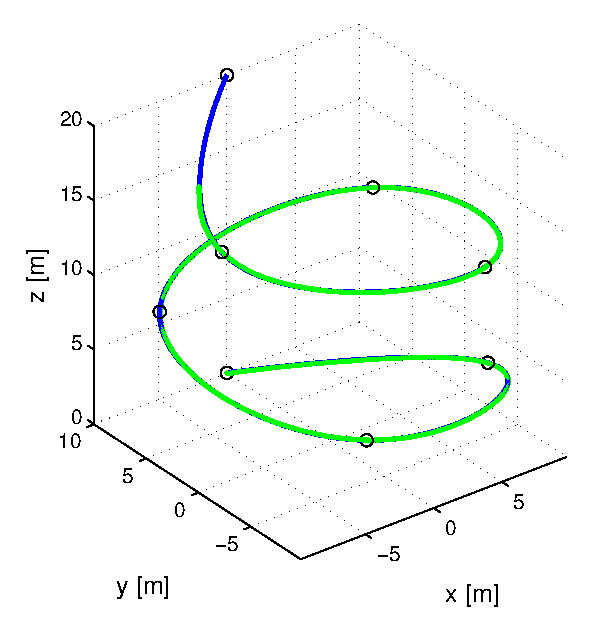
\includegraphics[width = \textwidth]{trackings_wc/figure_3D_helix_SplineDegree3_purePursuit_Disturbance_0}
  \end{minipage}
  \hfill
  \begin{minipage}[t]{0.32\textwidth}
    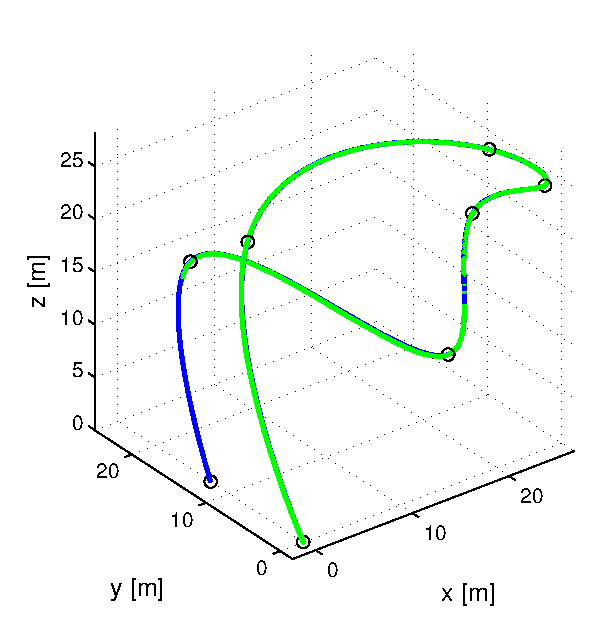
\includegraphics[width = \textwidth]{trackings_wc/figure_3D_agile_SplineDegree3_purePursuit_Disturbance_0}
  \end{minipage}
  %\caption{BLA tracking }
  \vspace{5pt}
  \begin{minipage}[t]{0.32\textwidth}
    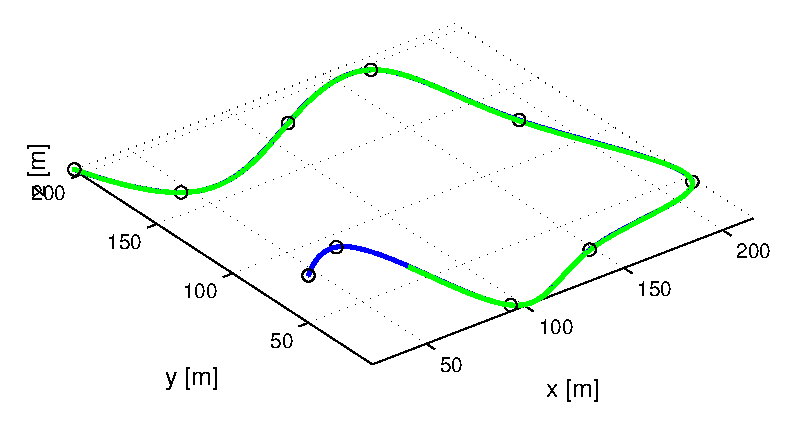
\includegraphics[width = \textwidth]{trackings_wc/figure_3D_road_SplineDegree3_crossTrack_Disturbance_0}
  \end{minipage}
  \hfill
  \begin{minipage}[t]{0.32\textwidth}
    \includegraphics[width = \textwidth]{trackings_wc/figure_3D_helix_SplineDegree3_crossTrack_Disturbance_0}
  \end{minipage}
  \hfill
  \begin{minipage}[t]{0.32\textwidth}
    \includegraphics[width = \textwidth]{trackings_wc/figure_3D_agile_SplineDegree3_crossTrack_Disturbance_0}
  \end{minipage}
  \caption{BLA tracking }
  \label{fig:results_model_uncertainties}
\end{figure}

We can show the results in a table, or we can put it all to the appendix..

\begin{table}[h]
\begin{center}
 \begin{tabular}{lll|lll}
 \hline
 Controller &   & unit & \textit{Road} & \textit{Helix} & \textit{Agile} \\ \hline \hline
 Trajectory Following & Av. Dev. & $[m]$ & 3.227 & 1.628 & 0.838 \\
 Pure Pursuit         & Av. Dev & $[m]$ & 3.650 & 0.098 & 0.037 \\
 Cross Track          & Av. Dev & $[m]$ &  0.034 & 0.061 & 0.023 \\
    
 Trajectory Following & Av. Acc & $[m/s^2]$ & 0.031 & 0.191 & 0.138 \\
 Pure Pursuit         & Av. Acc & $[m/s^2]$ & 0.031 & 0.136 & 0.121 \\
 Cross Track          & Av. Acc & $[m/s^2]$ & 0.028 & 0.140 & 0.120 \\
 \hline
 \end{tabular}
 \caption{Here some absolute results with model uncertainties.}\vspace{1px}
 \label{tab:absolute_results}
\end{center}
\end{table}

\section{Discussion}
\label{sec:discussion}


